\documentclass[11pt]{report}
\usepackage{graphicx}
\usepackage{subfig}
\usepackage{amsmath}
\usepackage{amssymb}
\usepackage{url}
\usepackage{bm}
\usepackage{setspace}
\usepackage[margin=2cm]{geometry}
\usepackage{epstopdf}
\usepackage{titlesec}
\usepackage{algorithm}
\usepackage{booktabs}
\usepackage{multirow}
\usepackage{wrapfig}
\usepackage[framed,numbered,autolinebreaks,useliterate]{mcode}
\usepackage[bookmarks,hidelinks,bookmarksnumbered=true,pdfstartview=FitH]{hyperref}

\newlength{\wideitemsep}
\setlength{\wideitemsep}{.5\itemsep}
\addtolength{\wideitemsep}{-7pt}
\let\olditem\item
\renewcommand{\item}{\setlength{\itemsep}{\wideitemsep}\olditem}

\newcommand*{\fullref}[1]{\hyperref[{#1}]{\ref*{#1} \nameref*{#1}}} % One single link
\newcommand{\HRule}{\rule{\linewidth}{0.5mm}}
\DeclareMathOperator*{\argmin}{arg\,min}
\DeclareMathOperator*{\argmax}{arg\,max}
\renewcommand{\vec}[1]{\boldsymbol{\mathbf{#1}}}
\doublespacing

\begin{document}

\begin{titlepage}
\begin{center}

% Upper part of the page. The '~' is needed because \\
% only works if a paragraph has started.
~\\[2cm]
\includegraphics[width=0.15\textwidth]{drawings/oxford.pdf}\\[1cm]

\textsc{\LARGE University of Oxford}\\
\textsc{\Large Department of Engineering Science}\\[1cm]

\textsc{\Large Third year project}\\[0.5cm]

% Title
\HRule \\[0.4cm]
{\huge \bfseries Detecting sleep apnoea via non-invasive methods}
\HRule \\[1.5cm]

% Author and supervisor
\begin{minipage}{0.4\textwidth}
\begin{flushleft} \large
\emph{Authors:}\\
George \textsc{Cochrane}\\
Tuan Anh \textsc{Le}\\
Sophie \textsc{Louth}\\
Sachin \textsc{Mylavarapu}
\end{flushleft}
\end{minipage}
\begin{minipage}{0.4\textwidth}
\begin{flushright} \large
\emph{Supervisor:} \\
Dr.~Frank \textsc{Payne}
\end{flushright}
\end{minipage}

\vfill

% Bottom of the page
{\large \today}

\end{center}
\end{titlepage}

\begin{abstract}
The abstract text goes here.
\end{abstract}

\tableofcontents

\chapter{Introduction (George)}
\label{ch:introduction}
% The division of labour among the group members is outlined in \fullref{ch:divisionOfLabour}.

Obstructive Sleep Apnea (OSA) is a highly prevalent condition worldwide and is understood to be linked with several causing factors, both biological and environmental. Diagnosis is currently attained after the patient visits a sleep laboratory; this process is costly both monetarily and in terms of the time required by specialists to carry out the full diagnosis. The main alternative diagnosis to this is by way of a home testing kit, but again this has an associated cost and requires some training before use.

This project explores the use of a smartphone app to provide a preliminary form of diagnosis which can then be provided to a General Practitioner to recommend whether a patient needs further tests and/or treatment. The project aims to remove the need for specialist knowledge to carry out the diagnosis and the clearest way to do this is by a non-intrusive technique. As the condition is characterised by distinctive snoring sounds, audio has been identified as a useful input to characterise OSA, along with the simple but effect method of a questionnaire to identify the disposition to known causal factors. The project is constrained by the commonly available hardware and software capabilities of smartphones. It looks to maximise the accuracy of the diagnosis using some advanced techniques of data handling, as well as discuss some of the detail pertaining to the physical implementation of a smartphone app.
\chapter{The Condition (Sophie)}
\label{ch:medicalInfo}
Obstructive Sleep Apnoea (OSA) - sometimes called hypersomnia sleep apnoea syndrome, occlusive sleep apnoea ~\cite{whitelaw1993characteristics}, sleep disordered breathing ~\cite{sleepdisorderedbreathing}, hyperventilation syndrome or Pickwickian Syndrome (although the latter three terms are discouraged because they are also used to describe other disorders)  - is a sleep disorder characterised by repetitive blockages in the upper airway during sleep, but with inspirational effort. These blockages can be apnoeas - full closure - or hypopnoeas  - partial closure. Both cause a restriction in airflow, which can lead to reduction in oxygen saturation and frequent arousal in order to re-establish airflow ~\cite{american2001international}.

The upper airways include the nasal cavity, oral cavity, and pharynx - the area behind the tongue (see Figure \ref{fig:Sagittal-Face}). Blockages mainly occur in the pharynx which is usually held open by the pharyngeal dilator muscles. Although these relax during sleep, in a healthy subject they are still able to maintain airflow, however in an OSA sufferer they provide insufficient force to prevent collapse ~\cite{fogel2004sleep}. Collapse only occurs during inspiration and is due to negative pharyngeal pressure. During rapid eye movement (REM) sleep there is further relaxation of the pharyngeal dilator muscle which can lead to longer apnoea and hypopnoea events. 

\begin{figure}[h]
\centering
\includegraphics[width=1\textwidth]{drawings/Sagittal-Face}
\caption{Sagittal View of the Face to show Upper Airways ~\cite{sagittalface}}
\label{fig:Sagittal-Face}
\end{figure}
Many factors affect the likelihood a patient suffers with OSA, however one thing is consistent in almost all cases; the pharyngeal upper airway size is smaller than in normal patients and often more elliptical, with the long axis directed anterior-posterior rather than laterally as it is in non sufferers, which alters the pharyngeal dilator muscle orientation leading to a mechanical disadvantage. This can have a number of causes including fat deposits and facial bone structure ~\cite{leiter1996upper}. 
Overweight and obese patients often have fat deposits lateral to the pharynx, not always substantial, but their positioning creates or reinforces elliptical shape, pharyngeal orientation and reduction in size. 

The main element of facial bone structure that influence upper airway size is the positioning and size of the maxilla and mandible (upper and lower jaw bones), these can influence the airway size in two ways: micrognathia where the jaws are undersized, and retrognathia (or overbite) where the mandible is set back compared to the maxilla. In both of these cases the tongue sits further back in the mouth, increasing the tendency to block airflow. Lower positioning of the hyoid bone and Brachycephaly, where the head is wider than it is tall, can have a similar effect ~\cite{lowe1995cephalometric}.

Abnormal facial tissues can also have an effect; large tonsils and adenoids, elongated or enlarged uvula (the dangly bit at the back of the mouth, see Figure \ref{fig:Anterior-View-Mouth}), macroglossia (enlarged tongue), high arched or narrow hard palate, and reduced nasal patency (cross sectional area), possibly caused by nasal abnormalities, all have been shown to factor ~\cite{schwab1995upper}.

\begin{figure}[h]
\centering
\includegraphics[width=0.8\textwidth]{drawings/Anterior-View-Mouth}
\caption{Anterior View of the Mouth to show Upper Airway Tissues~\cite{anteriormouth}.}
\label{fig:Anterior-View-Mouth}
\end{figure}

Other factors include lying supine (on one’s back) where gravity causes the tongue to fall into the airway. Some drugs including alcohol relax the pharyngeal dilator muscles more than just the effects of sleep, worsening OSA. Smoke irritates tissues including those in the upper airways, swelling them causing a narrowing of the airway ~\cite{apneosotherfactors}.

 Severity of the Condition can be measured in two ways: AHI and RDI. AHI or Apnoea Hypopnoea Index counts the average number of apnoeas and hypopnoeas per hour asleep. The severity is then classified as minimal if AHI \textless\ 5, mild if 5 $\leq$ AHI \textless\ 15, moderate 15 $\leq$ AHI \textless\ 30 and severe AHI $\geq$ 30. RDI or Respiratory Disturbance Index is similar but also includes respiratory-effort related arousals (RERAs) in the count ~\cite{AHI}. The same classifications are used for RDI as for AHI; however this can be unhelpful given that the RDI is likely to be higher than AHI for the same patient ~\cite{epstein2009clinical}.


\chapter{Rationale}
\section{Medical Rationale (Sophie)}
\label{sec:medicalneed-sophie}
Medical rational for the app can essentially be split down into two areas: prevalence i.e. how many people suffer; and prognosis, likely course of the condition. There is additional supporting evidence for a preliminary diagnostic app for obstructive sleep apnoea, some of which is discussed below

The British Lung Foundation has prioritised OSA and created an OSA Charter calling on the UK governments to make OSA a national priority as well as encouraging investment in research. They held a three year campaign to raise awareness which ended in 2014. The campaign had two aims: to increase awareness by both the general public and health care professionals and to improve diagnosis. Part of the plan to improve diagnosis was to develop a national standard for diagnosis that would include a “one-stop shop for treatment set-up [to] shorten the total patient pathway, especially from diagnosis to treatment, [to] reduce concerns about driving”. A conference on OSA was held in February 2014 where doctors expressed a desire to change the current system, due to increased need for doctor referral of patients to sleep centres ~\cite{britishlungfoundation}.

PhysioNet and Computers in Cardiology, with funding from Margret and H.A. Rey Laboratory for Nonlinear Dynamics in Medicine, set up a competition with two prizes of \$500 for whoever could classify ECG data, obtained minimally intrusively and inexpensively, into that from OSA sufferers and normal subjects, with the intension of using it as a screening tool ~\cite{physionet}.

The Agency for Healthcare Research and Quality felt that the diagnosis of sleep apnoea was a sufficiently important public health issue that they commissioned a study on future research needs which includes a reference to the need for portable monitors, including limited-channel, low-cost portable devices ~\cite{balk2012future}.

\subsection{Prevalence}
Prevalence of OSA is hard to know due to the fact a high levels of cases go undiagnosed (up to 90\% of cases~\cite{finkel2009prevalence}), however estimates range from 1 to 28\% of the adult population depending on severity and location ~\cite{young2002epidemiology}.

There may be an ethnicity element in prevalence, however few studies have been undertaken other than in western countries and therefore prevalence elsewhere is essentially unknown. For some areas it is known, this means studies on causes can be undertaken. For example prevalence in Western Nations and Hong Kong is very similar but prevalence of risk factors is very different: there are high levels of obesity in the west but not in those studied from Hong Kong, so hypotheses have been produced on other risk factors including facial features being more prevalent in Hong Kong and some clinical observations support these hypotheses ~\cite{ip2001community}.

Gender has been shown to have an effect with estimates of 2 to 3 times greater risk for men compared to women; the reasons behind this are unclear ~\cite{strohl1996recognition}. Hormones have been considered but administration of the female hormones oestrogen and progesterone to men does not appear to have an effect ~\cite{shaver2000review}. Men show greater prevalence to many chronic diseases so this may be part of a greater trend and differences elsewhere have been shown to be linked to physical features, occupation, environment, attitude to health, and risky behaviour. There are gender differences in upper airway shape, muscle activity, facial shape, and deposition of fat in the airway, however the few studies that have looked at this have yet to find a conclusive link. Occupation, attitude to health and risky behaviour have not been studied in the context of gender disparity in OSA sufferers ~\cite{waldron1985we}.

There are hypotheses proposing higher prevalence of OSA in pregnant mothers but few data sets to support this. Proposed mechanisms to cause this include excess weight gain and the effect of sleep deprivation on pharyngeal dilator muscle activity ~\cite{franklin2000snoring}.

Although a positive correlation between OSA prevalence and age appears to exist for mid life, the same is not true for younger or older patients. OSA in children has similar consequence to that in adults and some of the pathophysiology (physical manifestation of the disease) is the same, however the etiology (causes) and associated morbidity (rate of incidence of the disease) can be very different, which means that it is generally studied independently from the adult form ~\cite{ancoli1991sleep}.

In old age prevalence of OSA increases, however this does not necessarily mean that physiological changes associated with old age are causing OSA. If this was the case one would expect the prevalence rate to increase at the same rate as through middle age or at a higher rate. Figure \ref{fig:prevalence} shows the Sleep Heart Health Study on prevalence with age which starts to flatten in the 60s which suggests age related prevalence tails off at this point ~\cite{young1996sleep}.

\begin{figure}[h]
\centering 
\includegraphics[width=0.5\textwidth]{drawings/prevalenceage}
\caption{Prevalence of OSA by age in the Sleep Heart Health Study ~\cite{young2002predictors}.}
\label{fig:prevalence}
\end{figure}

It is possible that older age OSA is actually distinct from that of middle age. Several studies support this theory, as many of the key symptoms of middle age OSA are not present in the old age version, including daytime sleepiness, obesity, decrease in cognitive function and hypertension. Snoring is also significantly less reported, however this could be caused by increase in bed partner hearing loss and death ~\cite{enright1996prevalence,young1996sleep}.

\subsection{Prognosis}
The prognosis for sufferers of OSA can be quite severe, with many suffering with secondary conditions such as hypertension. Cognitive function is also impaired and most suffer from daytime sleepiness which effects ability to drive and hold down a job.

There is an association between OSA and secondary hypertension (high blood pressure) independent of excess weight and other factors. This link is seen even in mild OSA, and given the prevalence of OSA could be having an impact on a significant proportion of those suffering with hypertension. However attempts to treat OSA in order to reduce hypertension have so far yielded unclear results ~\cite{pankow2000sleep}.

Hypertension is linked to cardiovascular and cerebrovascular disease, and given the link between OSA and hypertension, OSA will moderately contribute to the morbidity and mortality of these. There may also be direct links between OSA and cardiovascular disease however this has been less well studied. Whether treatment of OSA can improve cardiovascular disease has yet to be assessed ~\cite{he1988mortality}.

Daytime sleepiness is a primary feature of OSA and many studies have shown that treatment of OSA does reduce daytime sleepiness ~\cite{ballester1999evidence}. Studies have found a significant association between snoring and daytime sleepiness ~\cite{engleman1999randomized,stradling1991self}.

The effects of OSA on cognitive function is not fully understood. There are some population based studies which find weaker correlations than clinic based studies. This is probably due to the biased population who attend sleep laboratories. In one study OSA was significantly but weakly related to reduced psychomotor efficiency (a measure of coordination of fine motor control with sustained attention). This link was not explained by daytime sleepiness ~\cite{kim1997sleep}. In another study of self reported snorers a weak but significant association was found between OSA and neuropsychological function ~\cite{adams2001relation}. One suggested mechanism for reduction in cognitive function is due to oxygen starvation in the brain during apnoeas. This can change neurons especially in the hippocampus and right frontal cortex and so far has not seen improvement with treatment of OSA ~\cite{gale2004effects}.

There is no specific quality of life measure for OSA although one is being developed. However the SF-36, a general health-related quality of life measure, a short form of the Medical Outcomes Study, is in use. A couple of studies have found a linear association between severity of OSA and decrements on the SF-36 scales, showing undiagnosed OSA has a similar affect on quality of life to other chronic disorders of similar severity. However another study showed a threshold effect as severity of OSA increased, however a small sample size limits usability ~\cite{finn1998sleep,baldwin2001association}.

Patients with OSA have a higher vehicle crash rate than the general population. This has been shown by crash records, self-reports and performance on driving simulators. This is a significant issue because it puts the lives of everyone not just the sufferers at risk. Studies undertaken in clinic will over estimate rate of crashes due to selection bias, however there are population studies looking at those with undiagnosed OSA which also show a strong correlation, especially among men. Self-reported sleepiness was not able to explain the crash rate. This is concerning because it means those at risk are not able to recognise it within themselves and are therefore unable to take precautions to reduce risk ~\cite{findley1988automobile,findley1989driving}.

\section{Economic Rationale}

\subsection{Current Solutions}

	As is evident, sleep apnea, particularly obstructive sleep apnea (OSA)
affects a significant proportion of the population and is worthy of
attention. The current available diagnosis options for sufferers or
potential sufferers are limited, expensive, invasive and realtively
inaccessible. We outline below the most common sources of help and
diagnosis for potential sufferers:
	\begin{itemize}
	\item NHS - GP check-up, home devices and polysomnography (PSG)
	\item Commercial home-testing devices
	\item Other possible future options such as mobile sleep apps and non-contact
health sensing technologies
	\end{itemize}

\subsubsection{NHS}

According to the NHS guidelines, patients who believe they may be suffering from sleep apnea can schedule a visit to their GP. The GP will ask a few questions to determine the likelihood of apnea, along with a physical examination that includes a blood pressure (BP) test and a hypothyroidism test, to determine whether an underactive thyroid gland is the reason for the patient's tiredness. The patient can then choose if he/she would like to be observed for one night in a sleep
centre, or would like to be given a monitoring device to wear at home when sleeping. Those who opt for a home sleep study are required to visit the sleep centre at a convenient time to collect and learn how to use the portable recording equipment. These include breathing sensors, heart rate monitors and oxygen sensors. Information from the device can be analysed on the next visit and further action, such as referring to a sleep centre can be taken \cite{nhsmain,nhsdiag}.

Observation at a sleep centre is done through polysomnography (PSG). This involves electrodes being placed on the face, scalp and above the lips, and bands being placed around the chest and abdomen. Additionally, sensors are placed on the legs and an oxygen sensor is attached to a finger. The tests carried out during a PSG include:

	\begin{itemize}
	\item Electro-encephalography (EEG)
	\item Electromyography (EMG)
	\item Recording of thoracoabdominal movements
	\item Recording of oronasal airflow
	\item Pulse Oximetry
	\item Electrocardiography (ECG)
	\item Sound and Video Recording
	\end{itemize}

The data from these tests is used to positively diagnose obstructive sleep apnea and a treatment regimen is then decided upon and enforced by the healthcare professional \cite{nhsdiag}. For the purposes of this report, we shall not delve into the treatment of OSA - we concern ourselves with the diagnosis process and how we can improve it.


\subsubsection{Commercial home-testing devices}

While these devices are more commmon in the United States, they are also available in the UK, and can be purchased if desired without visiting a GP. An example of such home-testing devices is the AccuSom\textsuperscript{\textregistered{}} test from NovaSom Inc. \cite{novasom1,novasom2}, pictured below: 

\begin{figure}[!ht]
\centering
\includegraphics[width=0.5\textwidth]{drawings/Novasom}
\caption{AccuSom\textsuperscript{\textregistered{}} \cite{novasom2}}
\label{fig:Novacom}
\end{figure}

The prevalence of such tests in the U.S. points towards the increasing
unfeasiblity of sleep centre tests for simple diagnosis of OSA, and
is an indication of where the diagnosis process is headed in the future,
in the U.K. as well as around the world. The economic reasons for
the trend are clear. On average, a single night at a sleep centre
and the associated tests could cost from \$800 to \$3000 in the U.S \cite{wsjhometest}.
(figures for the NHS in the U.K. are more difficult to find, but should
be comparable) The home tests can be administered at a fraction of
that price, ranging from \$200 to \$600 \cite{wsjhometest}. Moreover, sleep centre tests
are extremely inconvenient for the patients, and hence should be administered
towards the later stages of the diagnosis process. The use of home-testing
devices also allows a larger percentage of the population to be able
to test for OSA, which is desirable given that around 5\% suffer
from undiagnosed OSA \cite{nhsmain}.


\subsubsection{Other options}

The trend towards greater user independence in OSA diagnosis is further
observed through two major related breakthroughs - the rise of mobile
sleep apps and the development of non-contact health sensing technologies.

The popularity of sleep monitoring apps in the iOS and Android App
stores illustrates an increasing interest among smartphone users in
their sleep patterns. Currently, such apps use the accelerometers
and microphones to detect movements and noises from the users while they sleep, and use relatively simple algorithms to determine which stage of sleep the user is in. In addition, some apps come with additional headsets or headbands that track electrical impulses and measure the user's activity more accurately. The alarm clock function is activated only when the user is in light sleep (within a reasonable time window) to ensure he/she is woken up feeling energised \cite{currentapps}. Some examples of such apps are:

\begin{itemize}
\item Sleep Cycle (iOS) - \$1
\item Sleep Bot Tracker (Android) - Free
\item Wakemate - \$60
\item Lark - \$99
\item Zeo Sleep Manager Mobile - \$99
\item Sleep Tracker Elite - \$149 
\end{itemize}

The development of non-contact health sensing technologies holds promise as well. Recently, Xerox and Manipal University Hospital in India announced a collaboration to develop such techonologies at Xerox's research centre in Bangalore \cite{xerox1, xerox2}. Using image and signal processing algorithms, the collaboration aims to determine health indicators in a non-invasive manner, and such that monitoring can take place remotely \cite{xerox1}. The clear trend of health monitoring towards non-invasive methods and the increasing use of algorithms to supplement health care and diagnosis efforts is set to gain even more momentum as healthcare professionals begin to embrace 'big data' \cite{bigdata}.

\subsection{Proposed App - Where it fits in}

The need for an app that is able to diagnose OSA from a mobile platform, using non-invasive techniques is clear from the current diagnosis solutions and trends. While there has been a shift towards cheaper home-testing devices before necessitating a visit to a sleep centre, the fact remains that even at \$200, these tests are not inexpensive. What if we could create a means for diagnosing OSA without the need for cumbersome and invasive sensors, that could be accessed by anyone with a smartphone, at a negligible cost compared to a home-testing system? Those who have doubts over their sleep habits, but are too busy for a GP visit and do not want to spend money unnecessarily on a home-testing system could try the app and move on to pursue the matter more seriously if the results from the app suggested a need to do so. Since machine learning algorithms will be used in the processing of the data, the app has the potential to continuously improve in accuracy and, eventually, could outperform the home-testing devices. The development of image processing technology that could remove the need for invasive monitoring, especially in neonatal care, by Manipal University Hospital and Xerox sets a precedent and raises the possibility of diagnosing OSA without the need for sensors being placed around the body.


\subsection{Advantages of proposed app}

The advantages of the proposed smartphone app, that will use machine learning algorithms to accurately diagnose OSA using non-invasive mobile phone sensors, are numerous. Firstly, such an app, if utilised as a precursor to home-testing systems and sleep centres, could result in significant cost savings for both the healthcare provider and the patient. From the point of view of the NHS, savings from performing polysomnographies only on those who really need it would be substantial. Moreover, some of the functions such as collecting information about the patient can be done through the app using questionnaires to save time for the doctors. From the point of view of the patients, not having to schedule visits to the GP for collecting and returning home-testing kits would result in a larger number of users for the app than would otherwise have been the case.
This brings us to another advantage of using the mobile app - accessibility. Given that 65 \% of people over 65 in the U.K. have OSA \cite{nhsmain}, along with a significant proportion of middle-aged men and women, and that the condition often goes undiagnosed, it is essential to reach out to as many users as possible. The best way to do so is through mobile phones. The number of smartphone users is projected to increase globally from 1.75 billion in 2014 to almost 2.5 billion by 2017 \cite{phoneusers}. The graph below highlights the growth of mobile phone users worldwide:

\begin{figure}[!ht]
\centering
\includegraphics[width=0.5\textwidth]{drawings/mobilephoneusers.png}
\caption{Mobile Phone Users 2012 - 2017 \cite{phoneusers}}
\label{fig:mobilephoneusers}
\end{figure}

This highlights the potential for the app, and smartphone-aided diagnosis in general, not just in the U.K. but in other developing countries as well, where access to a sleep centre may not be as readily available.

The advantage that the proposed app holds over existing mobile phone apps is that it is specifically for diagnosing OSA - it is meant for medical purposes as opposed to general sleep cycle monitoring. This means that it does not compete with the above-mentioned apps, but serves a distinct purpose which is not possible in the other apps. Moreover, the use of machine learning algorithms in the app means that there is potential for the app to improve in accuracy over time as the amount and quality of training data used is improved. With every update, the app can become better at diagnosing OSA using only non-invasive methods.

In conclusion, the rationale for the project to develop such an app is clear. If developed, the app is viable as a supplementary service by the NHS and can improve the diagnosis of OSA in adults in the U.K. dramatically by reaching out to a wider audience and simultaneously result in savings for the NHS. It can also be further developed for use internationally, by those in developing countries in the future.


\chapter{The app}

\section{Structure Of The App}
The app has been designed to have a very simple structure and layout so as to be immediately usable and comprehensible, even by those less technologically minded. Each activity branches from the main “welcome screen” activity, and upon completion of each activity, the user is the brought back to the “welcome screen” activity in order to select the next stage of the app to complete (see Figure \ref{fig:appStructure}).
\begin{figure}[ht]
		\centering
			\includegraphics[width=.9\textwidth]{drawings/App_nav.png}
		\caption{Navigation between home activity and other pages}
		\label{fig:appStructure}
	\end{figure}
\subsection{Home Activity}
The app loads into the home activity when it is first turned on. The user is welcomed to the app and given a brief explanation of how to use the app. Below this the user is presented with three buttons to launch the three other activities. 
\subsection{Questionnaire Activity}
The first task for the user to complete is the questionnaire, based on the eight STOPBANG criteria questions as detailed later in the ‘Design Process’ section of this report. Pressing the submit button then takes you back to the start page and simply stores the number of ‘yes’ answers the questionnaire received. This number is called during the processing of the overall results, noting that three or more ‘yes’ answers indicates a high risk of Obstructive Sleep Apnea. The default for all of the answers is ‘yes’ which should encourage the user to actively read/change each question (given that statistically the average person would have more ‘no’ answers). It also means that should the user bypass the questionnaire section or ignore the questions before hitting ‘submit’, the app will use the higher risk criteria and results will be more likely to suggest too high a probability of apnea than miss a positive diagnosis altogether. 
\subsection{Sound Analysis Activity}
This activity is indicated as the second task to complete, though it doesn’t require completion of the questionnaire before being executable itself. The user is presented with four simple buttons as seen below. Note the following button restrictions (Figure \ref{fig:recordPages}):
\begin{itemize}
\item `Stop' cannot be pressed until the phone is recording audio.
\item `View Data' and ‘Delete File’ do nothing until there is data stored (‘Nothing yet’ is displayed as an indicator’).
\item When `Start' has been pressed, the ‘Stop’ button becomes the only usable button. This is done by checking whether the inbuilt Boolean variable ‘isRecording’ is true, and as such, the inverse becomes true again as soon as ‘Stop’ is pressed.
\end{itemize}
\begin{figure}[ht!]
		\centering
			\includegraphics[width=.9\textwidth]{drawings/Audiorecord_struct.png}
		\caption{Buttons are disabled depending on whether recording is in process}
		\label{fig:recordPages}
	\end{figure}
(see Figure \ref{fig:recordPages})
For this simple prototype of the app, recording is restricted to one file in any instance of the app running.
\\ The sound data is automatically stored to a file accessible only by the app and is later analyzed by the machine-learning algorithm and overall results algorithm. Clearly the delete button is only included for cases where recordings were accidentally created and as such, it uses a comprehensive ``Are you sure?'' alert upon pressing to avoid deletion of wanted files.
\\Progress bars are used whilst the sound is being saved and loaded which will reassure the user that the app is still running properly during these otherwise unresponsive stages of high CPU usage. 
\subsection{Results Activity}
In this activity, a simple algorithm is used to determine an overall probability that the user has obstructive sleep apnea, and brief medical advice is given accordingly. It combines the results of the questionnaire and the audio recording analysis to do this, and therefore if one of these two parts is not present, it will ask for the user to go back and complete it before full results are displayed. Again, all analysis and loading tasks that takes more than half a second or so utilize a progress bar for improved user interface.
\subsection{Navigation Around The App}
The buttons are intended to be as intuitive as possible for navigation of the app. Loading each extra activity can only be done from the home activity, and the activity is exited by pressing the hardware ``back'' button whilst on the home activity (see Figure \ref{fig:nativeButtons}). Each extra activity exits back to the home activity upon pressing this ``back'' button too, though the Questionnaire has the same functionality added in to the ``Submit'' button which helps reassure the user that the button has indeed been pressed.
\begin{figure}[ht!]
		\centering
			\includegraphics[width=.5\textwidth]{drawings/android_buttons.png}
		\caption{The hardware buttons are also coded for intuitive navigation}
		\label{fig:nativeButtons}
	\end{figure}

\label{sec:app}

\chapter{Design Process}

\section{Diagnostic Methods}
There are four strategies used to approach diagnosis they are; the algorithmic method, pattern recognition method, hypothetico-deductive method; sometimes called differential diagnosis, and the exhaustive method. 

The algorithmic method uses flowcharts and algorithms to analyse data that are precise and reproducible for example vitamin B12 level in blood. One follows steps making decisions at preselected branch point based on the clinical data available. This relies on a flow chart for the illness and the illness to present in a relatively normal way. Abnormal presentation of an illness could easily lead to misdiagnosis. For example if an OSA sufferer is not overweight but instead has lateral peritonsular narrowing, they may well be missed by this method. 

The pattern recognition method, is best for conditions with distinct presentation, especially those which present regularly in the population. It is refered to as pattern recognition because the symptoms and signs displayed by the patient reawakens memories in the doctor of previous examples. It is an efficient method, especially useful when time critical diagnoses are needed. This does however risk jumping prematurely to a final hypothesis, although the consequences of this can be reduced by follow up in order to check instincts. 

The hypothetico-deductive method lends itself to primary care settings as it results in a differential diagnosis, a rank ordered list of hypotheses. Hypotheses are generated and rejected as more data are collected and questions asked until a working hypothesis is reached. This method is most often used as it reflects how most people deal with life, and is therefore the most natural. It can cause errors if a doctor has been exposed to a certain diagnosis recently, they may choose to ignore signs that what they are looking at is in fact not that. For example if a doctor has diagnosed and number of patients with OSA recently ( or read a paper about it) they may diagnose a patient who expresses day time sleepiness and witnessed apneas with OSA when in fact the previous traumatic head injury would be an indicator for Central Sleep Apnea, in this case a polysomnogram would be needed to see whether the patient was actually attempting respiration during apneas. Another error situation can be caused by the doctor failing to think about the probability of a diagnosis being correct. for example, if a patient presents with witnessed choking during sleep as the primary symptom rather than daytime sleepiness or witnessed apneas the doctor may diagnose Sleep Choking Syndrome however this has a much lower prevalence than OSA, rare compared to about 2-4\% for OSA.

The exhaustive method works on the premise of having all the information, all data collected, all questions asked. Completeness of data is important for hospitalised patients but acquiring it is too time consuming and expensive for most cases. Useful for unusual illness when other methods have failed or for unusual expressions of illnesses. 

The hypothetico-deductive method will be useful in order to establish what symptoms and signs can be used to differentiate OSA from other disorders. However the app itself will need to rely on pattern recognition because ruling out all options will be impossible as a doctor won’t be administering the app. It was also be unnecessary to use an exhaustive method as the app is only designed to pick up OSA not all sleep disorders or reasons for daytime tiredness. 

\section{Signs and Symptoms -- non-invasive methods}
Table X shows all the known signs and symptoms of OSA along with detectable presentation. From there Table X+1 shows these presentations and the different sensors for measuring them, as well as whether those sensors are invasive or not. The non-invasive sensors shall be the focus of the following work. The presenting symptom for OSA is daytime sleepiness, with reports of snoring and witnessed apneas from the patient’s bed partner. So focussing on other conditions with these symptoms is a start to finding a unique combination of symptoms for OSA that can be tested non-invasively by an app. 


Table X+2 looks at four key symptoms of OSA which the majority of patients display ( and can be detected non-invasively). Disorders which also display one or more of these symptoms are then listed along with their differentiator from OSA. From the table it is clear most of these conditions can be ruled out by diagnosis focussing on daytime sleepiness, snoring, and an apnea awakening/choking combination. 

Ascertaining these would eliminate all but central sleep apnea and altitude insomnia however both of these would be picked up a significant proportion of the time by a questionnaire because the sufferers would only fit the risk cases for OSA in a small percentage of cases. Especially for altitude insomnia as those with a BMI over 35kgm-2 are unlikely to be climbing over 4000m in height for extended periods ( i.e. climbing mountains rather than flying).

Those suffering from central sleep apnea are likely to reflect population distribution for BMI as weight is not a cause or exacerbating factor. I.e. about 25\% of central sleep apnea patients are obese ($\text{BMI} > 30$) compared to 70\% of OSA sufferers.

Methods are then needed to detect daytime sleepiness, loud snoring and apnea arousal (choking) combinations. Sensors to look at are; video, accelerometry, audio and questionnaires. Idea and their merits and weaknesses will be discussed next.

\subsection{Video}
The aim is to pick up on apneas via cessation of breathing and arousal via significant body movement. Snoring would not be possible to detect although some other attributes that hint at OSA may be detectable e.g. lying in the supine position ( on back). Video could also be used to detect sleep and activity, e.g. sleep cycle transitions and limb movements. 

Merits include, smartphone already have cameras so an external camera wouldn’t be needed, although the cameras may struggle with the low light level in the sleeping space, and changing the light level in order to accommodate the camera could have a knock on effect on the quality or type of sleep. 

Weaknesses include, positioning of the camera will be important and this is hard when all rooms are different and smartphones don’t naturally stand up by themselves. Manual analysis of the video has been used until recently so there isn’t a great deal of statistical data on how well computer algorithms can detect OSA. Video produces large data files that cannot be sensibly stored on a phone. Video has formed part of the polysomnogram in some areas for a long time as an aide to observation and only recently investigated as an independent method of diagnosis using automated analysis. As a consequence lots of video data does exist however it is highly regulated due to patient confidentiality. 

\subsection{Accelerometry}
This has the potential to be able to detect body position and sleep wake segmentation which could give a pretty good indicator of apnea arousal events, however mechanism for detecting snoring.

This has not been part of the polysomnogram although it has started to be investigated as a mechanism for detecting OSA. There is very little data available which makes a retrospective study a challenge, especially as there is no data conbined with polysomnogram data for verification. Positioning of the phone in order to get the best results without damaging the phone would require some investigation. Non standardised arrangements of mattress and bed clothes may cause issues. 

\subsection{Audio}
The most obvious way to detect audio signals from the patient is via the phone’s in built microphone although external microphones should also be investigated. It ought to be possible to detect apnea arousal events and snoring. 

Lots of work has been done on audio analysis of speech so there are lots of ideas out there to work from. Many polysomnograms include a sound recording for reference so there is a lot of data available and in the most part it is anonymised so there isn’t a risk to patient confidentiality. In some cases it has been labelled so it can be used easily for a retrospective study such as this one. There are also regulations which can act as a guidline. 

\subsection{Questionnaire}
A questionnaire is pretty much the only way to assess daytime sleepiness, it can also be used to acquire about other symptoms and co-morbidities. If a prexisting questionnaire is used then there will be data on its effectiveness and usability and statistics it has produced. Questions for part of the diagnostic pathway so it takes some of the work away from the doctor. Some studies show patients are more truthful with anonymous questionnaires than with their doctor, more on that to follow.

\subsection{Conclusion}
Given that audio analysis and questionnaires should be sufficient to diagnose OSA and rule out other similar disorders, these will be investigated further with the other methods discarded unless significant issues are encountered with audio and questionnaire analysis.

\newpage
\section{Questionnaire selection}
The key point that needs to be established via the questionnaire is whether the patient suffers from daytime sleepiness however knowing about the patient’s weight can be useful to eliminate central sleep apnea, and other questions about symptoms can be useful to reinforce diagnosis. 

\subsection{Own vs Pre-Existing}
There is a key decision between two options at this stage, to create a new questionnaire from scratch or to use a pre-existing questionnaire. A new questionnaire gives much more freedom as to what questions to ask in order to target particular symptoms and eliminate other disorders. It also allows for unique methods of analysis e.g. weighted questions rather than a simple threshold based on number of questions answered. Rigorous market research can be used to design the wording of the questions to maximise truthfulness and ease of interpretation, as well as number of questions and mechanism of answering. However this would be time consuming and an expert is question production is potentially needed. Data from patients would need to be collected via the questionnaire and other means in order to test its effectiveness. 
Using pre-existing questionnaire allows for quicker set up time as there will either be data available in order to validate the questionnaire or it will have already been validated. Some questionnaires are within the doctor’s guideline so time can be saved during consultation if they are already performed. Named questionnaires are often recognised by doctors which saves them time checking the questions and they are also more likely to trust questionnaire they know. 
Given the time constraints and the access to data and skills further investigation will look at pre-existing questionnaires. 

\subsection{How Truthful are People}
One of the benefits of performing questionnaires on the app rather than waiting for patients to attend an appointment is saving doctors time however there is another benefit in the form of increasing truthfulness. 
One study found that patients tended to lie in order to look good, in the context of sexuality, those involved had a strong interest in not giving a disappointing impression. 
Another study looked at doctors’ trust in patients which is an indicator of suspected lying. Ulterior motives were thought to have a significant influence on patients’ truthfulness. In the case of OSA there is a risk of patients playing down daytime sleepiness in order to avoid diagnosis if they wish to avoid having to contact the DVLA and their car insurance company and risk losing their license or insurance due to misunderstanding. There is also a case that patients may try and get a diagnosis in order to receive disability related financial support, however tricking a night time study into thinking you have OSA would be challenging. 

\subsection{Questionnaires}
There are a number of questionnaires that have been used to assess diagnosis of OSA, some rely on a doctor to measure physical features, others use characteristic clinical features, others use patients’ interpretations of their symptoms, and the rest use combinations of the above. 

\begin{itemize}
\item Viner et al\\
Model incorporates snoring, BMI, age and gender. Used stepwise linear logistic regression.
\item Maislin et al\\
Model incorporates snoring, gasping at night, witnessed apneas, age, gender and BMI. Multiple logistic regressions were used to generate a multivariable apnea risk register when compared to RDIs from polysomnographs. ROCs were used to test predictive ability. 
\item Metzer et al - Berlin Questionnaire\\
Model incorporates snoring, gasping at night, witnessed apneas, age, gender and BMI. Multiple logistic regressions were used to generate a multivariable apnea risk register when compared to RDIs from polysomnographs. ROCs were used to test predictive ability. 
\item Kirby et al – Artificial Neural Nets\\
Uses 23 clinical variables including patient’s history, physical examination and patient reported sleepiness and smoking.
\item Dixon et al\\
Looked at witnessed apneas, neck circumference and BMI. Study rather than a questionnaire. 
\item Kushida et al – Kushida Index\\
Complicated morphometric model, including BMI, neck circumference, palatal height and oral cavity measurements amongst others. Suffers from being too complicated to be administered accurately and being time consuming.
\item Tsai et al - upper airway physical examination protocol (UAPP)\\
Looked at six parameters, three clinical symptoms; snoring, witnessed apneas and hypertension and three measurable signs; cricomental space, pharyngeal grade and overbite ( info on these to follow)
\item Chung et al – STOP questionnaire\\
Four questions on snoring, daytime sleepiness, witnessed apneas and blood pressure.
\item Chung et al –STOPbang questionnaire\\
This is an extension of the STOP questionnaire that adds four additional questions on BMI, age, neck circumference and gender. A threshold of 3 out of 8 is generally used to indicate OSA. 
\item Meoli et al – AASM OSA exploratory questionnaire\\
This questionnaire is referenced in a number of places however there is no data to back it up
\item Chung et al – ASA\\
Three categories are used to ask questions, physical characteristics, observed sleep disturbances and tiredness. It uses falling into two or more of these categories as an indicator of OSA. 
\item Flemons’ et al – Flemons’ screening tool\\
This is a 36 question screening tool for OSA that uses a differential method for diagnosis, asking questions about depression and chronic diseases as well as the more common questions on tiredness, snoring and driving behaviour. Uses a weighted score called SACS with a threshold to indicate OSA. 
\item Johns – Epworth Sleepiness Scale\\
A questionnaire using eight questions to assess sleepiness in different situations. Recommended by NHS guidelines. 
\end{itemize}

\subsection{Narrowing Down the Studies}
A number of these aren’t formal questionnaires and therefore not known by the doctor negating one of the reasons for using a pre-existing questionnaire, however this isn’t sufficient reason to rule them out. The Kushida Index and ASA questionnaire are complicated which goes against the design specification. A high negative predictive value is needed so the focus of more work will be on; Artificial Neural Net, UAPP and the STOPbang questionnaire. Epworth Sleepiness Scale will also be included in the app because it is part of the diagnostic pathway as laid out by the NHS.

\section{Audio}

\subsection{Scoring of apnea R\&K vs AASM}
Audio signals taken during polysomnograms are currently scored by sleep specialists, there are two guidelines as to how to do this. The Rechtschaffen and Kales Manual is long standing, it was the only manual in use between 1968 when it was created and 2007 when the AASM Manual came into use. 
The R\&K manual is based on healthy subjects aged 21 to 86 years and doesn’t actually mention how to recognise apneas. It has also been criticised for being open to interpretation. The AASM manual has a slight change in terminology and changes distribution of NREM sleep stages but the main difference is it explains how to classify more sleep abnormalities including apneas and arousals. 
The AASM scores a signal as an apnea if, there is a drop in the peak thermal sensor excursion by more than 90\% of baseline, the event last at least 10 seconds and at least 90\% of the event’s duration meets the amplitude reduction criteria for apnea. Obstructive apnease are associated with continued or increased inspiratory effort through the period of absent airflow. A minimum desaturation criterion is not required. 
The basis for scoring arousals is based on EEG and EMG and therefore isn’t helpful in terms on how to analyse audio signals. 

\subsection{Methods of Analysis}
There are a number of different methods that can be used to analyse audio signals, each will be looked at in turn, looking at how they work, studies on them and strengths and weaknesses of the method. Due to issues with background noise and other signal noise most methods focus on the characteristic snores of OSA sufferers rather than the quiet apneas. 

\subsubsection{Simple Characteristics}
Three simple features of a snore can be analysed quite easily, snore duration, the time taken for a snore sound, generally measured in seconds; snore loudness, generally the average loudness measured from a microphone, a snore simulator is also needed in order to calibrate the microphone; snore periodicity, calculated from segmented short frames of the snores with low amplitude, high frequency components removed, autocorrelation used to asses each frame as either periodic or not. Overall periodicity calculated from the ratio of the number of periodic frames to the total number of frames.

Jones et al studies these features amongst others in order to see whether it was possible to predict the outcome of palatal surgery rather than as a diagnostic measure for OSA. Frame size of 200ms was used centre-clipped by 30\%. Autocorrelation peaks between 25 and 87.5ms were used to classify as periodic. 

\subsubsection{Peak Power}
Using Fast Fourier Transforms a power spectrum can be created of the snores. This can then be characterised in a number of ways including establishing: Fa the fundamental frequency; Fo the lowest frequency, Fpeak the peak with the maximum power, Fmean the statistical mean frequency, and Fmax can also be calculated, however there are different conventions for this, it is defined as the frequency beyond which the signal amplitude has dissipated to less than a percentage of its peak power, some studies use 3\% others 1\%. 
Perez-Padilla et al used Fa, Fo, Fpeak and Fmax to examine the differences between nine OSA sufferers and ten simple snorers. Defining Fmax as dissipating to 3\% of peak power. Sound was recorded via a microphone attached to the manubrium sterni (chest). Significant variation was found between snores in a given patient making it hard to find a differentiator between OSA sufferers and simple snorers. It was found that for OSA suffers Fpeak was usually at a higher frequency than Fa, however this was significant enough to be used to differentiate the two groups.

Fiz et al used Fpeak, Fmean and Fmax defined at 10\% of peak power to distinguish between ten OSA sufferers and seven simple snorers. The microphone was placed just above the larynx without skin contact. Two features were found to distinguish OSA sufferers from simple snorers. The first was peak frequency (Fpeak) which was significantly lower in OSA sufferers with a threshold of 150Hz, although one of each group was on the opposite side, a strong non linear negative correlation was seen between Fpeak value and number of AHI events as seen in figure X ( 3), this is associated with a Spearman rank order correlation: r=-0.70; p<0.0016. The second feature was to do with the shape of the power spectrum. The simple snorers displayed a clear fundamental frequency and harmonic pattern whereas the OSA sufferers displayed a low frequency peak with scattered peaks over a narrow band of frequencies, Figure X (1 \& 2 b) shows the different patterns. Fiz et al attributed the differences seen to microphone placement, Perez-Padilla et al placing their microphone on the chest whereas Fiz et al placing above the larynx, this results in a different filtering effect caused by the different tissues and cavities the sound travels through. 

\subsubsection{Power Ratio}
Given the difference in spectra between those with OSA and simple snorers there is potential to characterise this by means of a cumulative power ratio. This would be the area under one part of the power spectrum divided by the area under the rest, where the threshold(s) is placed would depend on what characteristic was trying to be differentiated. From the power spectrum from the Fiz et al study above one potential threshold would be 100Hz to pick up on the low frequency components of the OSA curve, see figure X ( adapted version of 1\&2 b from Fiz). 
Perez-Padilla et al used superimposed spectra from ten snores from each subject (9 OSA, 10 simple snorers) and a threshold of 800Hz, dividing the integral of the spectra above 800Hz with that below 800Hz, for OSA patients who took a second breath after an apnea the cumulative power ratio was also calculated for that. Figure X (8) shows the scattering of the ratios, with snorers having a ratio of 0.08 $\pm$ 0.02 and OSA sufferers a ratio of 1.12 $\pm$ 0.31. A threshold of 0.3 was proposed which would distinguish all but one OSA sufferer on first breath after apnea, this patient had a low AHI and mild symptoms. 
Hara et al used the same method as above on 46 OSA sufferers and 12 simple snorers, keeping the threshold at 800Hz, using a ratio of below 800Hz to above 800Hz. Simple snorers had a power ratio of 34.002 whereas OSA sufferers had a ratio of 6.288. The p value of a Mann-Whitney U test was 0.015, this small value is a good indicator that this didn’t happen by chance. 
Hara et al wouldn’t recommend this approach as the calculation is very time consuming. Significant differences were found between the values of the ratios in both studies although in both cases a difference between OSA sufferers and simple snorers was clearly seen. 

\subsubsection{Sound Intensity}
Another diagnostic tool uses sound intensity without frequency, instead looking at the apnea-snoring combination. Define an acoustic signature event (ASE) as a period of apnea, duration specified between limits, followed by snoring, where snoring and apnea are defined in terms of sound intensity.
Van Brunt DL et al define apnea below 50microV and snoring above 100microV with apnea episode lasting between 10 and 90 seconds. 30 second intervals were analysed by sound intensity and polysomnogram and analysed in two ways. Firstly each patient (69 patients, 51 OSA suffers, 18 not) was assessed independently and RDI score compared with predictions, for an RDI of 15/hour or greater sensitivity was 0.93, specificity 0.25, false positive 36.2\%, false negative 2.8\%, 60.9\% classified correctly. Secondly pooling all the observations (60231) resulting in a 33\% sensitivity, 98\% specificity, 85\% classified correctly. 

\subsubsection{Formants}
Formants are the resonant frequencies of the signal, most easily determined by picking out the peaks on a linear predictive coding (LPC) spectrum of the signal. LPC is the spectral envelope produced by a linear predictive model. The lowest formants are associated with degree of constriction of the pharynx, degree of advancement of the tongue and degree of lip rounding respectively, these are often referred to as F1, F2 and F3. Because these physical properties change in sufferers of OSA there is a chance that the frequencies associated with them will change too, therefore threshold frequencies to distinguish OSA sufferers and simple snorers are sought. 

Ng et al tested 30 OSA sufferers and ten simple snorers and found a threshold for F1 of 470Hz but not F2 nor F3, this threshold yielded a sensitivity of 88\% and a specificity of 82\%. However increased sensitivity and specificity were seen if different thresholds were used for men and women as seen in table X (1). Women show a greater distinction in F1 frequency than men as well as a reduced spread of results, although more outliers amongst the simple snorers, as seen in figure X (1). It is however worth noting that the sample size for women was small (6 OSA sufferers, 4 simple snorers) Once the threshold has been established an equation is needed to convert it to an AHI value, a number of equations were proposed and regression used to see which was the best fit, as seen in table X(2). A power law came out best with a regression of 0.5334 giving a predicted AHI score of 12.2 when 10 was being aimed for. It is worth noting that the same subjects was used for training and testing, although different data for each.

Sola-Soler et al used formant frequencies to distinguish between snores from eight simple snorers ( 447 snores) and eight OSA sufferers ( 236 normal snores and 429 post-apneic snores). The spectral envelope was estimated by linear predictive autoregression, with very low amplitude spurious peaks rejected by a 3dB threshold. Investigation of the spectral envelope found 2 to 6 formants in each snore, these fell in common frequency range around 150Hz, 500Hz, 1KHz, 1.7KHz, and in a few snores 2.2KHz. This led to definition of five frequency bands: B1[0,300), B2[300,700), B3[700,1400), B4[ 1400,1900) and B5[ 1900,2500) in Hz. For each band and type of snore ( simple snorer SN, OSA normal snore OP-N, and OSA post apneic snore OP-PA) the mean value Fi and standard deviation SFi was calculated. Table X (3) shows a comparison between these means and standard deviations for each combination of snore type calculated using the Mann-Whitney U test, the fifth band was left off because so few snores exhibited this formant. If a snore had more than one formant in a band the average frequency of those was used in the calculation. Bands 1 \& 3 showed significant differences between formants when comparing the standard deviation of simple snorers and OSA sufferers both in normal snores and post apneic snores of the OSA sufferers. The most distinct difference was between the standard deviation of simple snorers’ normal snores and post-apneic snores in band 1 which had a probability of 0.0006. 

Yadollahi et al used formant frequencies to distinguish between snores and breaths rather than simple snorers and OSA suffers so a direct comparison of method cannot be made however there is value in exploring the method used. Bands were used as in the Sola-Soler study but at different frequency ranges, [20−400]Hz, [270−840]Hz, [500−1380]Hz, [910−1920]Hz, [1680-2680]Hz, [2580-3770]Hz and [3590-5000]Hz these were found using K–means clustering. This is a method of partitioning data unsupervised, it uses an iterative method to find a predefined number of partitions, in this case seven, an error margin of $10^{−5}$ was used for the iterations. The process is sensitive to initial conditions so was repeated 20 times with different initial conditions, the one with the minimum error was selected. Table X (3) shows the student t-test p values, which show the first and third formants to be significant, with probability p = 0.003 and p = 0.0244 respectively. The F1 frequency of the breath sound was greater than that of the snore while the F3 frequencies with the converse. 

\subsubsection{Bispectral Analysis}
Bispectral analysis exploits the fact that the bispectrum reveals both amplitude and phase information about a spectrum, while also being calculated by convolution makes it the easiest polyspectra to compute. Polyspectra are Fourier Transforms of cumulants, for example the second order cumulant; autocorrelation Fourier Transforms to the Power Spectrum. The third-order cumulant C(m,n) = E{x(k)x(k+m)x(k+n)} transforms via a Double Discrete Fourier Transform (DDFT) to the bispectrum . Although the bispectrum is often plotted on a square it is symmetric and so only a triangular region is needed to completely describe it, this is defined by $0 \le \omega2 \le \omega1, \omega1 + \omega2 \le \pi$

Quadratic phase coupling occurs uniquely in second-order non-linear systems, and is where the phases add and subtract along with the frequency components. (QPC) causes peaks in the bispectrum triangular region, this shows energy is produced at frequency $\omega1 + \omega2$, a flat bispectrum at w1 and w2 suggests no activity and that it is not affected by QPC. 

Ng et al exploited the bispectrum shape in order to distinguish between nine OSA sufferers and seven simple snorers. Bispectral analysis has benefits over power spectrum because it reveals the non-Gaussian and non-linear behaviour, given the upper airway is non-linear this is a good plan. 

Noise was suppressed using a level-wavelet-dependent (LWD) thresholding scheme under undecimated discrete wavelet transform (UDWT) setting. Fast Fourier Transforms were used to estimate the bispectrum, this was plotted (figures X and X (4 \& 5) and inspected visually, the axies have been normalized with a frequency of 1 being 11025Hz. From visual inspection is appears the biggest peak for simple snorers are near the origin while for apneic snores are further away, this suggests a greater degree of phase coupling in apneic snores due to nonlinearities in the signals. When analysed peak position was reflected in the numbers with apneic peaks are higher frequencies than simple snore peaks, table X(1) shows the figures.

Clustered multiple comparison graphs were then produced, figure X(6), QPCs appear mainly at $f_1=f_2$ for simple snores whereas they appear mainly at $f_1 \not= f_2$ for apneic snores, however there is less self coupling. 77\% of simple snore are self coupled compared to 49\% of apneic snores. So the analysis shows there are three differences between simple snores and apneic snores, apneic snores have strong presence of nonlinear interaction, less self-coupling and QPC peaks appear and higher frequencies. 

\subsubsection{Wavelet Analysis}
Translation-Invariant Discrete Wavelet Transform(TIDWT) is a nonorthogonal, undecimated adaption of the more common Discrete Wavelet Transform (DWT) which is orthogonal and maximally decimated, and causes Gibbs like artefacts around discontinuities. There are two TIDWT methods:`a-trous and cycle-spinning. The `a-trous scheme removes the downsamplers and upsamplers of the DWT and upsamples the filter coefficients by a factor of $s^{j-1}$ in the $j^\text{th}$ level of the algorithm. As the output of each level contains the same number of samples as the input it is inherently redundant. 

Cycle spinning incorporates translation invariance by applying DWT to all circular shifts of the input vector and averaging over them. However due to periodic properties the number of shifts reduces to one. Both schemes offer better error properties than DWT due to redundant coefficients by about 10-20%. 

Ng et al used cycle spinning TIDWT to distinguish between 30 OSA sufferers and ten simple snorers. Ten snores of about 6 seconds were randomly chosen from each snorer, marked by polysomnogram technologists. Figure X(5) compares the energy approach used by Cavusoglu et al and the TIDWT approach used by Ng et al in this study. At the narrowest tolerance of 25ms the TIDWT approach detected 51\% of the snore segments correctly compared with 8\% for the energy approach, and at the largest tolerance of 125ms the TIDWT approach detected 98\% correctly, whereas the energy approach only managed 87\%, i.e. the TIDWT approach is at least 10\% more effective. 

\subsubsection{Multiscale Entropy Coefficients}
Entropy is used as a measure of complexness and the idea of using entropy for multiple scales was originally proposed by Zhang however this was based on Shannon’s definition of entropy that has some flaws so Costa et al proposed a new method using sample entropy (SampEn) a refinement on approximate entropy (ApEn) introduced by Pincus .

The method works by constructing consecutive coarse-grained time series of the original time series. These are created by averaging the data points within non-overlapping windows of increasing length. Each element of the coarse-grained series is calculated by the equation . An illustration of this is shown in figure X (1)

SampEn is then calculated for each coarse-grained time series and plotted as a function of the scale factor. SampEn quantifies the regularity and predictability of the time series, it acts as a regularity statistic, looking for patterns, it does this by looking at the probability that m consecutive data point that are similar will remain similar when one more data point is added, here similar means the distance between them is less than r. 

Roebuck and Clifford used MSE over 40 scales (1-40seconds) to distinguish between 50 simple snorer, 72 OSA sufferers and 24 normal subjects. They used 240minutes of recording from each subject, splitting the data between a training set and a testing set 70:30. Scales of 6seconds, 21seconds and 30second yielded a specificity of 92.5\% and a positive predictive value of 85.8\% in the training set and a specificity of 90.5\% and a positive predictive value of 83.5\% in the testing set.


\newpage
\section{Signal Analysis -- simple method}
\label{sec:simple-sachin}

\subsection{Outline}

The simple method of diagnosing sleep apnea, using audio data from the user's phone that is recorded while he/she is sleeping, was meant to provide a starting point for the development of the app. It served three main purposes:

\begin{itemize}
\item To familiarise us with the typical sleep patterns and with power and frequency content of sleep data
\item As a backup\\
This would give us a method that is able to provide a diagnostic output such as the apnea-hypopnea index score from sleep data, even if it was not using machine learning algorithms. 
\item As a point of comparison\\
The simple method would serve as a point of comparison, along with other methods used, with regards to the accuracy of the diagnosis. Using simple metrics such as percentage accuracy of pre-determined apnea or hypopnea points in the data against what the model is able to pick out, we can compare the simple model results with our machine learning results. This would allow us to gauge our preformance and also prove that the app is able to diagnose OSA with superior accuracy.
\end{itemize}

MATLAB\textsuperscript{\textregistered{}} was used as the development environment for the simple model. This was due to several reasons. Firstly, our familiarity with MATLAB\textsuperscript{\textregistered{}} from previous projects made it a natural starting point. Secondly, as a dynamically typed language with a user-friendly interface, MATLAB\textsuperscript{\textregistered{}} would enable us to make minor changes to the code and observe the results quicker. Experimentation and tinkering with the code is much easier in MATLAB\textsuperscript{\textregistered{}}  than it is in C/C++ or Java, for example. This ease of experimentation meant that MATLAB\textsuperscript{\textregistered{}} is a good language to start writing the model in, and is used in the initial development of the machine learning HMM model as well. With in-built functions such as audioread, MATLAB\textsuperscript{\textregistered{}}  provided the basic tools with which we could develop the model. Of course, if necessary, the model could later be written in Java for implementation in an Android App - this would be trivial.

The MATLAB\textsuperscript{\textregistered{}} code for the simple model is presented below, with detailed explanations. A brief summary is as follows: three .m files are created - simple.m, the main script which is is run once an audio file is created and stored, and  two functions detectApnea.m and detectApneaVar, that take a vector of the signal power and a few other parameters as inputs. The simple.m script uses the wavread or audioread function (the user's audio sleep data is recorded in .wav format) to read the file and produce a matrix of the audio level values. This is sampled at a lower frequency in order to reduce memory storage. The frequency content of the signal is calculated using the fast fourier transform function (FFT) Along with a plot of the signal, a plot of the frequency content is generated (this is done purely for the programmer's convenience and analysis). The power content is calculated from the signal vector and is used in the detectApnea function. An additional function, detectApneaVar, is included in the code below highlighting two different ways of analysing the data. The first way, used in detectApnea, uses a simple threshold parameter, and searches the signal power vector for prolonged periods of time when the value is below a threshold level. These periods represent apneatic episodes when the user's airflow experiences blockages. The second way, used in detectApneaVar, aims to identify the sudden inspiration that accompanies the body attempting to re-establish airflow. This is usually characterised by a snorting noise from the user. Instead of simply looking at the power values and comparing them to a threshold, detectApneaVar identifes periods of high variance in the signal, which represent the user being `shocked' to start breathing again.

\subsection{Implementation in MATLAB\textsuperscript{\textregistered{}}}

\begin{lstlisting} 
% Reading data
clear all;
close all;
FILENAME = 'signal.wav';
[YRaw,f] = audioread(FILENAME) ;
TMAX = length(YRaw) / f;

% Sampling data because we don't need very high resolution
scale = 20;
for i = 1:(length(YRaw) / scale)
    Y(i) = 0.5 * (YRaw(i * scale, 1) + YRaw(i * scale, 2));
end

% Plots sampled data
figure;
plot(Y);
title('Sleep signal');

% Calculates and plots frequency
N = length(Y);
Yf = fft(Y,N);
freq = ((0:1/N:1-1/N)*f).'; % Frequency vector;

% Plot spectrum.
plot(freq,abs(Yf)) 
title('Amplitude Spectrum of y(t)')
xlabel('Frequency (Hz)')
ylabel('|Y(f)|')

% Calculates and plots the power
power = Y.^2;
\end{lstlisting}

The first part of the code above assumes that the user's sleep data has already been recorded using the microphone and has been stored in a file \'signal.wav\'. This file is read using the wavread function as mentioned, and outputs YRaw, a two-column matrix (as wav encoding uses two channels) as well as f, the sampling frequency which is 44.1 kHz. The length of the audio file in seconds, TMAX, is also calculated for later use.

A sampling frequency of 44.1 kHz is unnecessarily large and wasteful for an application such as ours - the frequency content of a 7-minute sample obtained from YouTube \cite{simplevideo} is shown below. The figure on the left represents the spectral density while that on the right represents the information on a logarithmic scale so as to highlight where the useful information is found. As can be seen, there is no useful information that can be found at frequencies above 5 kHz (the duplicated spectra on the left are a result of sampling at the frequency of 44.1kHz). There is no risk of aliasing occuring even if the audio is sampled at 5 kHz. This is where the scale parameter in line 9 above comes in - it reduces the size of YRaw by sampling the already sampled vector(and also combines the two channels into one by taking the average). 

\begin{figure}[htb]
	\centering
	\subfloat[Amplitude Spectra of Raw Audio File]{%
		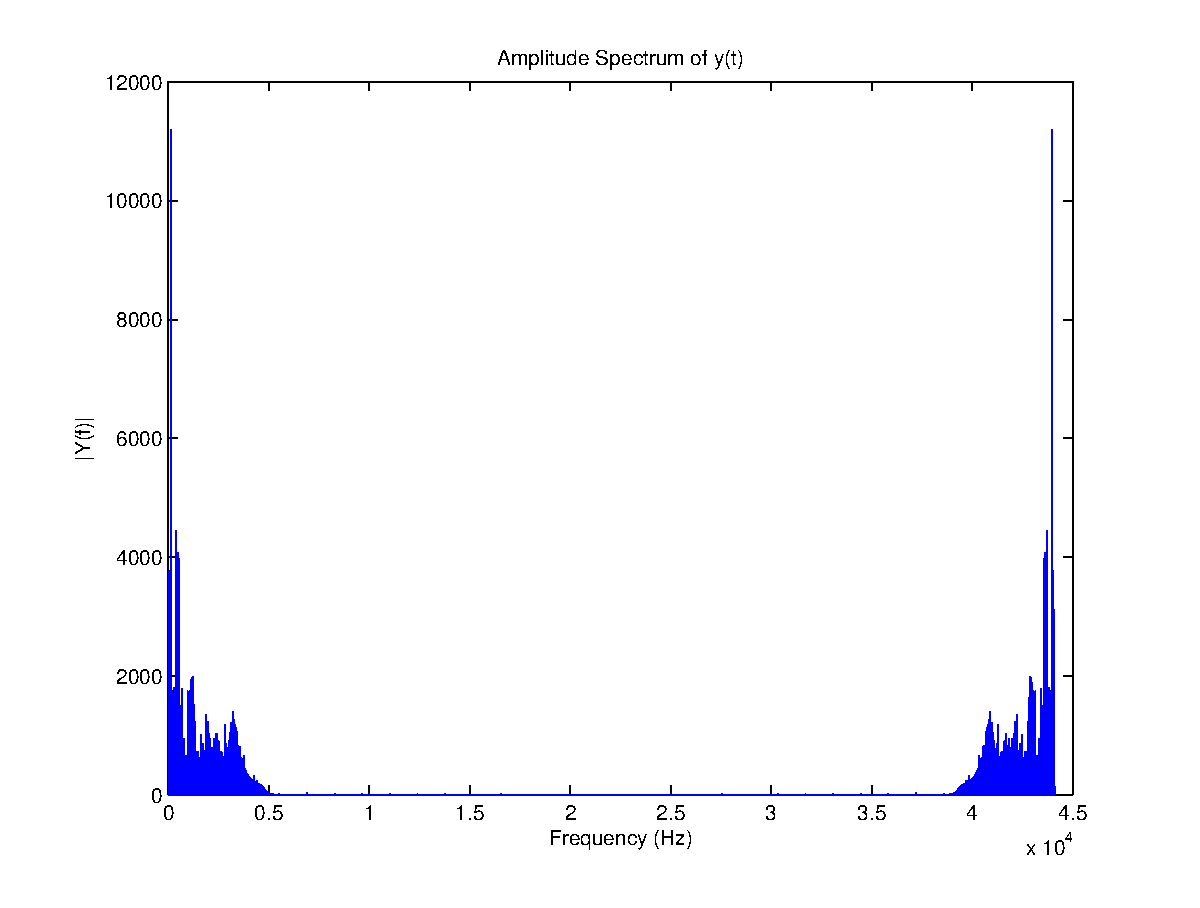
\includegraphics[width=.5\textwidth]{drawings/YRawFreq}}
	\subfloat[Periodogram of Raw Audio File]{%
		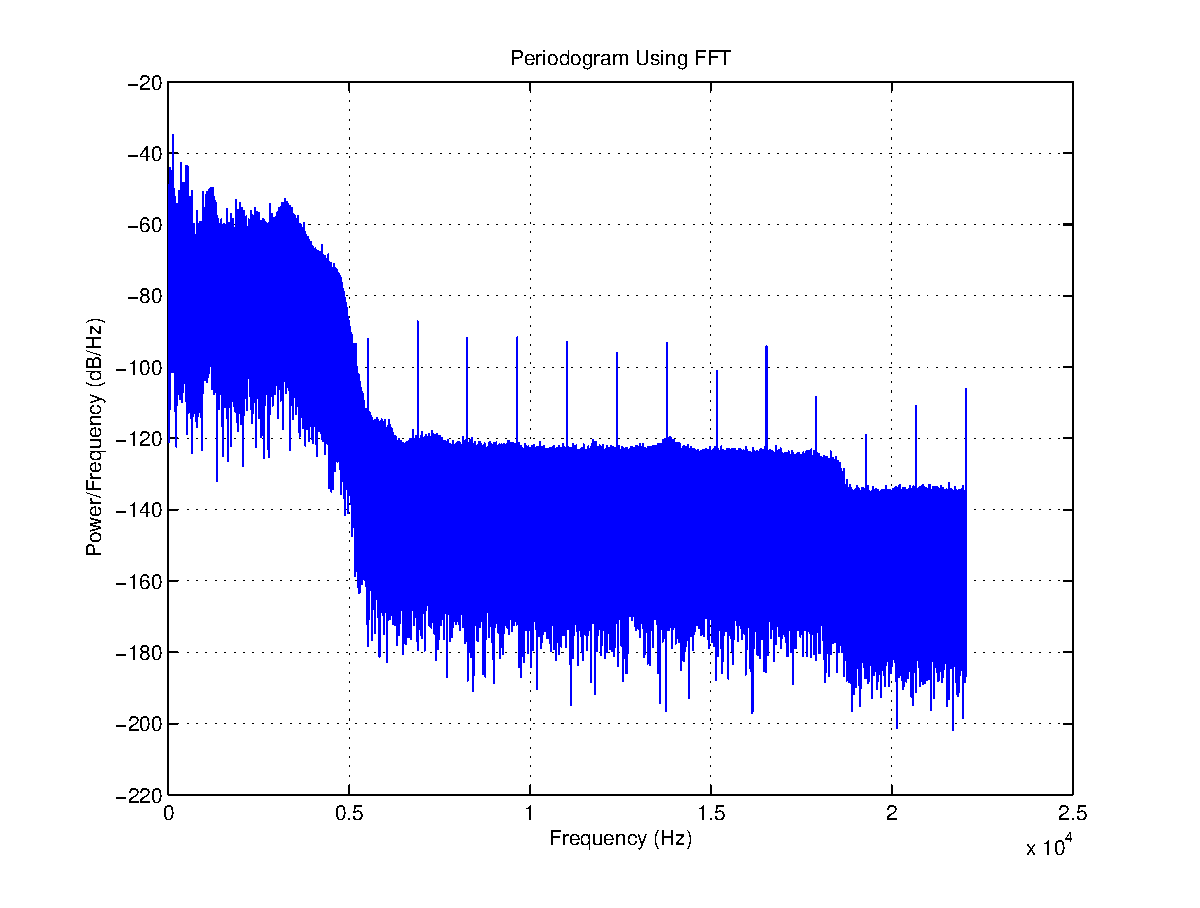
\includegraphics[width=.5\textwidth]{drawings/YRawPeriodogram}}
	\caption{Frequency content of Raw Audio File}
	\label{fig:simpleRawFreqContent}
\end{figure}

The frequency content shown above is calculated using the fast fourier transform (FFT) function in MATLAB\textsuperscript{\textregistered{}}. The function calculates the discrete fourier transform (DFT) of a vector $\vec x = \{x_1, x_2, \dotsc, x_{N}\}$ and returns output $\vec X = \{X_1, X_2, \dotsc, X_{N}\}$  such that
\begin{equation}
X(k) = \sum_{j=1}^{j=N}x(j)\omega^{(j-1)(k-1)}_N
\end{equation}

where

\begin{equation}
\omega_N = e^{(-2\pi i )/N}
\end{equation}

The next few lines of code above serve to calculate and plot, again, the frequency of the reduced vector Y (the figures above are for YRaw). The vector power is also created to hold values for the power of the signal at each time period, and will be used in the functions detectApnea and detectApneaVar.

The next part of the script sets some parameters and uses detectApnea as well as detectApneaVar to analyse the signal power. The results are then put together and plotted for the programmer's benefit. (The code for doing so is not shown here as it is relatively straightforward and unimportant)

\begin{lstlisting}
% Apnea detection
sensitivityMean = 0.01;
interval = 3;
sensitivityVar = 5e-2;
windowSize = 20;
apnea = detectApnea(power, TMAX, sensitivityMean, interval);
apneaVar = detectApneaVar(power , TMAX , sensitivityVar , windowSize);
\end{lstlisting}

The function detectApnea takes as inputs the vector power, the length of the audio file TMAX, and parameters sensitivityMean and interval. The code for detectApnea is shown below:

\begin{lstlisting}
function apnea = detectApnea(Y, TMAX, sensitivityMean, interval)

    n = length(Y);    % No. of samples
    sampleInterval = round(n / TMAX * interval);
 % Minimum no. of consecutive samples that should be below threshold for apnea
    apnea = zeros(1, n);
% Generate a vector that will contain either zeros or ones to show where apnea is
    
    threshold = mean(Y) / sensitivityMean;
    
    nBelowThreshold = 0;    % Number of sample points below the threshold in a row.
    for i = 1:n
        if Y(i) <= threshold
            nBelowThreshold = nBelowThreshold + 1;
% Increase # of sample points below the threshold in a row
        else   % We see a point that is above threshold.
            if nBelowThreshold >= sampleInterval    % Condition for which we classify apnea.
                for j = max((i - nBelowThreshold), 1):(i - 1)
% Loop through the last 'nBelowThreshold' points. Making sure (i - nBelowThreshold) doesn't go below 1 (otherwise error).
                    apnea(j) = 1;
                end
            else
                for j = max((i - nBelowThreshold), 1):(i - 1)
                    apnea(j) = 0;
                end
            end
            nBelowThreshold = 0;
        end
    end
end
\end{lstlisting}

Taking inputs sensitivityMean and interval, detectApnea runs through the vector power and identifies when the signal power is below a threshold level for at least a certain interval. This threshold level can be adjusted by changing sensitivityMean, and also is affected by the mean value of the overall signal power. This is important, as it is a first step towards ensuring that variations due to users putting the phone further away, which would reduce the overall power of the signal, are taken care of to some extent. The output vector apnea contains ones and zeroes at every sample point, with ones representing apnea  or hypopnea episodes.

Instead of simply searching the vector power for values lower than a threshold, detectApneaVar attempts to identify periods when there is a sudden spike in the signal power, which means the user has snorted and been shocked into breathing again. Similar to detectApnea, detectApneaVar uses parameters such as sensitivityVar and windowSize. The code for detectApneaVar is presented below:

\begin{lstlisting}
function apnea = detectApneaVar (Y , TMAX , sensitivityVar , windowSize)

n = length (Y);
apnea = zeros (1 , n);

% Calculate variance of whole signal (as a yardstick)
variance = var(Y) ;
maxVariance = variance / sensitivityVar;

% Calculate the variance through a moving window
twindow = [1:windowSize ; Y( 1:windowSize )];
% This vector contains the locations of the moving window

for i = 1:( n-windowSize )

    sigma2 = var( twindow(2, :) );
    
    if sigma2 > maxVariance 
        apnea(1 , twindow(1,:) ) = 1;
    end
    
    twindow(1,:) = twindow(1,:) + 1; % Update the window for the next round of variance calculations
    twindow(2,:) = Y ( twindow(1,:) );

end
\end{lstlisting}

As can be seen, a variance method is used to detect sudden spikes in the signal. A moving window is created of size windowSize and is used to temporarily house parts of the vector power. The variance of the values in the window is calculated and if it exceeds a value maxVariance, the user is recognised as having had an apnoeatic episode. The window moves on to the immediate next period after updating the output vector apnoea, and by the end the vector apnea contains ones and zeros identifying points in the signal where apnoea is thought to have occurred. Once again, variations due to different users and settings have been accounted for to a certain extent by calculating the value of maxVariance from the variance of the entire signal.

The results from the two methods of detecting apnoea are combined together, and the results are plotted below for the sample YouTube video. Firstly, the plot of the power signal, with peaks at regular intervals, confirms that the user has OSA and experiences apnoea and hypopnoea in predictable cycles. The results from the two methods are plotted below the power signal, and exhibit enough correlation such that combining the methods can be justfied. 

\begin{figure}[htb]
\centering
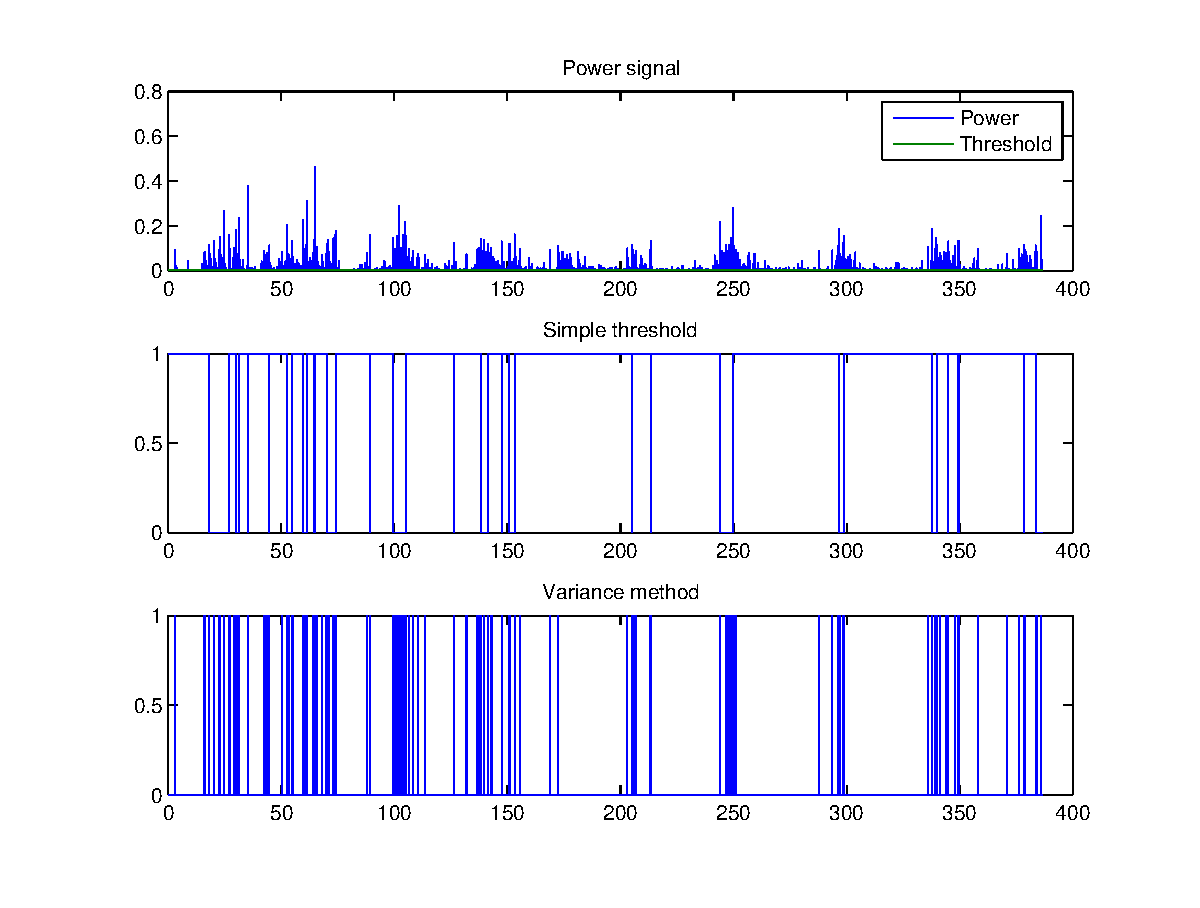
\includegraphics[width=1\textwidth]{drawings/simpleResults}
\caption{Diagnosis Results from 7-minute Sample}
\label{fig:simpleResults}
\end{figure}

\subsection{Limitations of model}

While the simple model we have used above gave us a good starting point and will serve as a point of comparison, it has many limitations. Firstly, the choice of parameter values plays a huge role in the accuracy of the diagnosis. Even though some effort at reducing the effect of variations in noise and signal strength has been taken, the choice of sensitivityMean, sensitivityVar, interval and windowSize is still arbitrary to a large extent. This means that while the model works well for the sample above, there is no guarantee of its effectiveness for other audio signals.

This is where machine learning comes in - needing to choose arbitrary parameter values is removed as the program can be designed to learn, with training data, the best values for parameters and update itself accordingly. The parameters do not have to be the same as those above, of course - this would depend on the exact machine learning model being used.

Secondly, the simple model assumes the existence of an audio file that has already been recorded. Given the average sleep time for adults of seven hours, this could lead to memory storage issues in smartphones where the recording is meant to take place. Some form of compression of the data needs to take place even while recording, and this issue is tackled in the following sections of the report.

\newpage
\section{Machine Learning -- Theory}
\label{sec:mltheory-ta}
	Machine learning, a branch of artificial intelligence, concerns the construction and study of systems that can learn from data \cite{wiki:machineLearning}. The supervised classification problem in machine learning concerns finding the unknown target function that classifies certain input data into classes based on some set of training examples containing labelled input data.

	It is exciting to use machine learning algorithms to aid medical diagnoses because it can dramatically save time for medical experts. These techniques should create a reasonably reliable, though not perfect, system on which the medical experts can base their decisions on.
	
	In our case, given a sampled sound signal of a sleeper, we want to identify apnoea periods. In particular, we represent our input (sampled sound signal) as $\vec S = \left\{s_1, s_2, \dotsc, s_T \right\} \equiv \left\{ s_i \right\}_{i = 1}^{T}$, and we want to output the classifiers for every $K$ samples, $\vec Y = \left\{ y_i \right\}_{i = 1}^{T/K}$, where the classifier $y_i \in \left\{0, 1\right\}$ corresponds to samples $\left\{ s_j \right\}_{j = \left(i - 1\right)K + 1}^{iK}$ of the signal. We assume that $T$ is divisible by $K$, however if this is not the case, we discard an appropriate number of signal samples to fulfill this condition.

	We have researched three models for our problem which we will discuss in this section. Firstly, we will discuss Support Vector Machines which are one of the most widely used algorithms in Machine Learning today, then we will discuss the State-Space Model and the Hidden Markov Models, which are more well-suited to our problem due to their temporal nature. Moreover, we discuss techniques to condition our data before using them as input data for our learning models.
	
\subsubsection{Support Vector Machines}

\paragraph{}
	Here, we present the theory for Support Vector Machines (SVMs) based on the lecture notes from Prof. Andrew Ng \cite{ng13}. SVMs are one of the most widely used and many argue among the best "off-the-shelf" supervised learning algorithms. This is mainly due to the sound theoretical framework, efficiency and good generalisation guarantees even for high-dimensional and linearly non-separable data.
	
\paragraph{Notation}
	Having $m$ training examples, where
	
	\begin{itemize}

  		\item $\vec{x}^{(i)} \in \mathbb{R}^d$ is the $d$-dimensional $i$-th training data.
  		\item $y^{(i)} \in \left\{-1, 1 \right\}$ is the $i$-th training label.

	\end{itemize}
	
	we want to find the parameters $\vec{w} \in \mathbb{R}^d$ which describe the hyperplane $\vec{w}^T \vec{x} + b = 0$ that separates our two classes. Thus, we can define our classifier as $h_{\vec{w}, b}(\vec{x}) = g\left(\vec{w}^T \vec{x}\right)$, such that $g(z) = 1$ if $z \geq 0$ and $g(z) = -1$ otherwise. Note that this is a non-probabilistic learning model as we are not considering the probability of each class or the data.
	
\paragraph{Objectives}
	The main intuition behind SVMs is that 
\subsubsection*{State-Space Models}

\paragraph{}
	
\subsection{Hidden Markov Models}

\paragraph{}
	Here, we present the Hidden Markov Models (HMMs), one of the most popular statistical models in machine learning with applications in many fields including but not limited to Crytanalysis, Speech recognition and Bioinformatics \cite{wiki:HMM}. The material is based on \cite{rabiner1989tutorial}, \cite{ramage07} and \cite{mlBook}. We will first present HMMs with discrete observations, then we extend this to include models with continuous observations.
	
\subsubsection{Discrete observations case}
\paragraph{}
	Similarly to SSMs, we have two sets of random variables. Observed variables $\{ y_t \}_{t = 1}^T$ which are drawn from the observation alphabet $V = \{v_1, \dotsc, v_M\}$, and hidden states $\{ x_t \}_{t = 1}^T$ which are drawn from the hidden state alphabet $S = \{ s_1, \dotsc, s_N \}$. The probabilistic graphical model of the HMM is identical to the one in Figure \ref{fig:pgm}. The hidden states obey Markov assumptions, i.e. $P( x_t | x_{t - 1}, \dotsc, x_1) = P(x_t | x_{t - 1}) = \text{const.}, t = 2, \dotsc, T$. Moreover, the observed variables are only dependent on the corresponding hidden state, i.e. $P( y_t | x_t, \dotsc, x_1, y_{t - 1}, \dotsc, y_1) = P(y_t | x_t), t = 1, \dotsc, T$.
	
\paragraph{}
	We parameterise a HMM using the transition matrix $\vec A$, emission matrix $\vec B$, and the initial state distribution $\vec \pi$. The transition matrix $\vec A \in \mathbb{R}^{N \times N}$ describes the transitions between hidden states, $A_{ij} = P(x_{t + 1} = S_j | x_t = S_i)$. The emission matrix $\vec B \in \mathbb{R}^{N \times M}$ describes the probability of an observation conditioned on a hidden state, $B_{jk} = P(y_t = v_k | x_t = S_j)$. The initial state distribution $\vec \pi \in [0, 1]^N$ simply describes the initial probabilities of the hidden state, $\pi_i = P(x_1 = S_i)$. The model is fully described if we know these parameters, which we group into what is called a parameter set of the model $\lambda = (\vec A, \vec B, \vec \pi)$.
	
\paragraph{}
	The three main questions of a HMM are
	\begin{enumerate}
		\item Find the probability of observations given the model, $P\left(\{y_t\}_1^T; \lambda\right)$.
		\item Find the most likely series of hidden states $\{x_t\}_1^T$ to have generated the observations $\{y_t\}_1^T$, $\widehat{\{x_t\}_1^T} = \argmax_{\{x_t\}_1^T} P\left(\{y_t\}_1^T | \{x_t\}_1^T; \lambda\right)$.
		\item Find the parameters $\lambda$ to maximise $P\left(\{y_t\}_1^T; \lambda\right)$.
	\end{enumerate}
\subsection{Conditioning input data}
\paragraph{}
	Working in the time domain, the data is usually transformed to the frequency domain to analyse where the pattern is found more easily. Also, whichever model we choose to use, we will work in high dimensions which means we need a lot of input data in order to find the pattern. In the case of SVMs, it will be high-dimensional training points $\{\vec x^{(i)}\}_1^m$, in case of SSMs and HMMs, it will be the high-dimensional observed variables $\{\vec y_t\}_1^T$. Thus, we will present two ways to condition the input data, before analysing it using the Machine Learning algorithms above. We use spectrograms to do the frequency analysis and Principal Components Analysis to reduce the dimensionality of the data.
\subsubsection{Spectrograms}
\paragraph{}
	

\subsubsection{Principal Components Analysis}
\paragraph{}
	

\subsection{Summary}
	We have explored the theory behind three models: Support Vector Machines (SVMs), State-Space Models (SSMs), and Hidden Markov Models (HMMs). While the SVMs model data discriminatively, the SSMs and HMMs do it generatively. In our project, we will use SVMs and HMMs to learn from actual sleep data and use the learnt model to classify unseen test data. We compare the performance of both methods by comparing the proportion of correct classifications.

	We have also discussed two methods to condition our data: using spectrograms and Principal Components Analysis (PCA). In our experiments, we will transform our data into spectrogram space and then perform PCA to choose only a few principal components to reduce the dimensionality of our data.

	The model with the best performance, together with the conditioning methods will be implemented in Java for Android integration.

\newpage
\section{Machine Learning -- Experiments}

\paragraph{}
	We obtained the data from the ECG database from the PhysioNet database located at \url{http://physionet.org/physiobank/database/apnea-ecg/}. The data consists of 35 labelled training records and 35 unlabelled records (used for the CinC Challenge 2000 competition). The recordings vary from less than 7 hours to 10 hours each and include continuous digitised ECG signal and, in the case of the training data, a set of apnoea annotations derived by human experts. The continuous signal is sampled at the rate of 100 Hz and the annotations are available at every 6000 samples (i.e. every minute) of the signal indicating the presence of apnoea at that time. One such record is shown in Figure \ref{fig:visualiseData}.

	\begin{figure}[ht!]
		\centering
			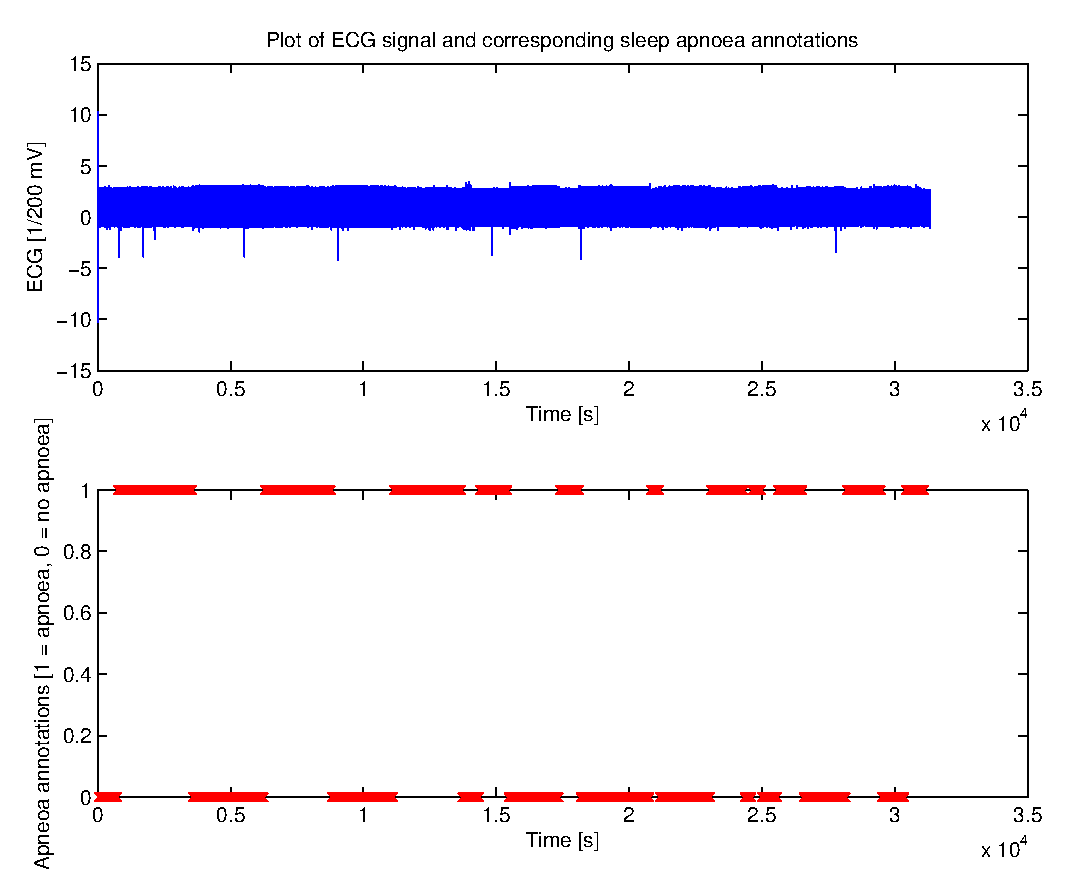
\includegraphics{drawings/visualiseData.eps}
		\caption{One training record}
		\label{fig:visualiseData}
	\end{figure}

\subsection{Reading and Conditioning Data in MATLAB}
\label{sec:RandCDatainMATLAB}

The code used for the training and testing of the data can be found in Appendix \ref{ch:HMMCode} for ease of explanation. Firstly, we examine the main script, covering the reading and conditioning of data, spectrogram transformation and PCA analysis. After explaining the various functions created and used in the script till then, we move on to cover the training and testing of the data.

From the code found in the Appendix \ref{sec:apneaHMM}, the \verb!trainIndex! and \verb!testIndex! vectors are used simply for selecting the files to be used, out of 35, for training and the remainder (or less) for testing the accuracy of the diagnosis. Having chosen the files, the next step is to extract and read the files. This is done using the \verb!readData! function, presented in Appendix \ref{ch:readingDataCode}.

The function reads data from the indices specified in \verb!fileIndex! (which is trainIndex in the main script above), and returns O, containing all the observations merged together in a TxD matrix. T is the total number of minutes of data, and D is the number of samples in a minute (6000 in this case), such that there are T annotations in total. The function also returns the vector q, a Tx1 vector containing the latent states for every minute in O, as well as consolidated time, signal and annotation time vectors for ease of plotting and analysis later on.

Firstly, \verb!readData! uses a simple function \verb!getFilenames! to return a 35x1 cell of the available filenames, in a cell string. Then, after initialising the variables, \verb!readData! uses a for-loop to run through each file and extract the relevant information. Using the pre-provided \verb!rdsamp! and \verb!rdann! functions, the signal values as well as annotations are read from the file. As the annotations use `A' for apnoeatic episodes and `N' for non-apnoeatic episodes, the vector type is converted to the alphabet ${0,1}$. The \verb!O! and \verb!q! output matrices are built up using the information from each file, and finally some trivial conditioning is done to ensure ease of plotting if the signal were to be kept.

Armed with the consolidated vectors \verb!X! and \verb!Y!, we now proceed to use the \verb!spectrogram! function in \verb!MATLAB!\textsuperscript{\textregistered}, as described in section~\ref{sec:conditioningExperiments-ta}. We then use the \verb!pca! function from the \verb!pmtk3! package to perform Principal Components Analysis (choosing the number of principal components we wish to include, \verb!k!). 
\subsection{Conditioning input data}
\label{sec:conditioningExperiments}

\subsubsection{Frequency Analysis}
	We use \verb!MATLAB!\textsuperscript{\textregistered}'s function \verb|spectrogram|, which takes the following parameters
	\begin{itemize}
		\item \verb!X! -- our signal $\vec x = \{x_1, x_2, \dotsc, x_N\}$.
		\item \verb!WINDOW! -- length (in number of samples) of the window $T_\text{window}$. The windows are automatically filtered using a Hamming window. We arbitrarily choose the window to be the number of signal samples corresponding to one annotation (6000 in our case).
		\item \verb!NOVERLAP! -- number of overlapping samples between two consecutive windows. Effectively $T_\text{window} - T_\text{offset}$. We arbitrarily choose the offset to be 1000 such that we have six bins of PSD's for each annotation.
		\item \verb!NFFT! -- number of frequency points used to calculate the discrete Fourier transforms. We use default.
		\item \verb!Fs! -- sampling frequency in Hz. In our case 100 Hz.
	\end{itemize}

	A spectrogram for one record can be seen in Figure \ref{fig:visualiseSpectrogram}. Just by looking at the spectrogram, we can spot different regimes of the time series (most clearly seen at $0.5 \times 10^4$, $1 \times 10^4$, $2 \times 10^4$, and $2.7 \times 10^4$ seconds). Comparing this to the apnoea annotations in Figure \ref{fig:visualiseData}, these regimes are actually the non-apnoeatic regimes. Also, we can see that most of the ``action'' is happening below 20 Hz. For this reason, we cut off the frequencies above 25 Hz for subsequent analysis. We combine the corresponding six bins of PSD's per annotation in to a large feature vector corresponding to that annotation. Next, we will reduce the dimensionality of these feature vectors using PCA.
	\begin{figure}[ht!]
		\centering
			\includegraphics[width=.5\textwidth]{drawings/visualiseSpectrogram.eps}
		\caption{Spectrogram of one record}
		\label{fig:visualiseSpectrogram}
	\end{figure}

\subsubsection{PCA}
	For this, we use the function \verb!pca! from the package \verb!pmtk3!. Once we get the principal components (orthogonal bases) and their corresponding principal coefficients (variances of the data, projected onto that base, correct to a constant factor) $\{\lambda_1, \lambda_2, \dotsc, \lambda_D\}$, we will plot the graph of their cumulative sum over their total sum $\frac{\sum_{i = 1}^n \lambda_i}{\sum_{j = 1}^N \lambda_j}$ in order to decide on the number of principal components needed. The plot is in the Figure \ref{fig:visualisePca}. Performed on the first 10 records, we can see that we will need to include at least 100 to capture half of the variance but at least 3000 components to capture the whole variance.
	\begin{figure}[ht!]
		\centering
			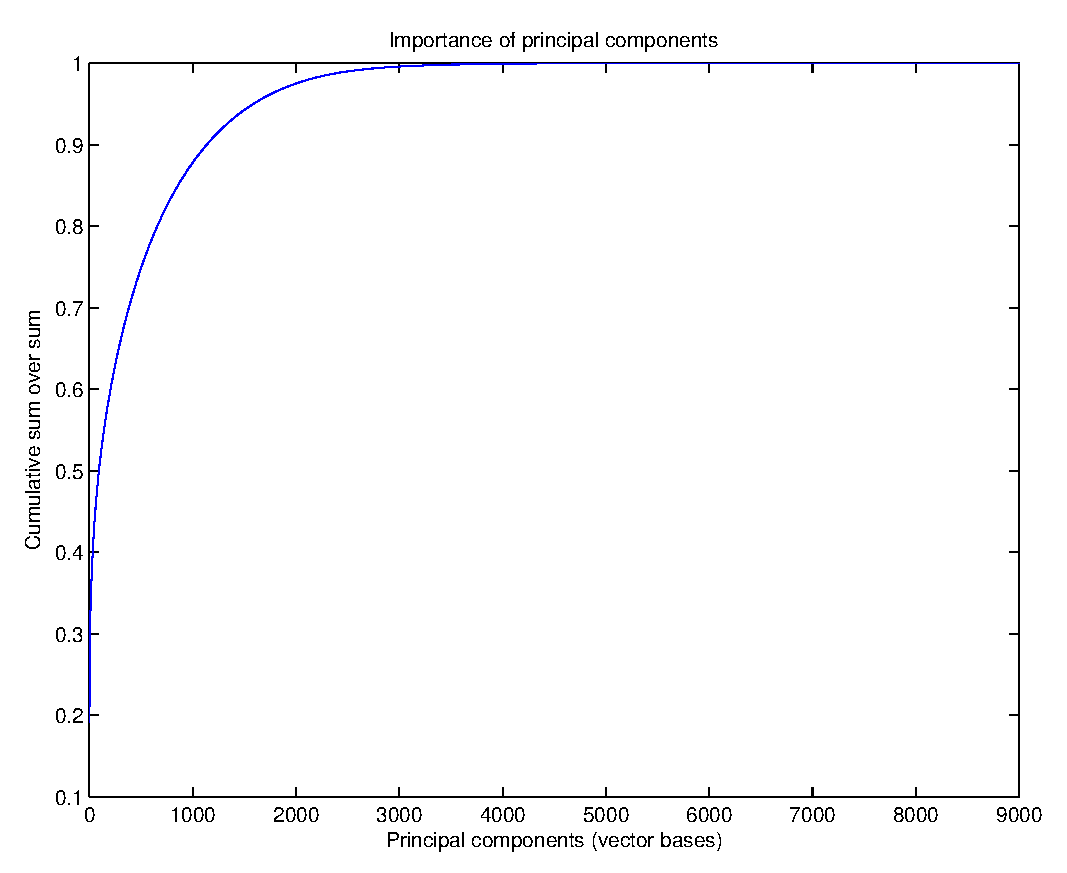
\includegraphics[width=.5\textwidth]{drawings/visualisePca.eps}
		\caption{PCA of the first 10 records}
		\label{fig:visualisePca}
	\end{figure}
\subsection{Data Visualisation}
	It is helpful to visualise our data to confirm the presence of any detectable patterns and/or to help improve our learning algorithms. Since our Principal Component Analysis revealed that we need at least 100 principal components to capture at least half of the variance, it is not illustrative to visualise our data by plotting the data points on a 2D plane using only the first two principal components. Instead, we take the six corresponding bins of spectrograms of the two classes of annotations (apnoea, no apnoea) and take the average for each class as shown in Figure \ref{fig:spectrogramClassesVisualise}. We can notice the differences in the spectrograms which is reassuring because we can see that there exist some patterns to be found and that the spectrogram contains enough information to detect sleep apnoea.
	\begin{figure}[ht!]
		\centering
			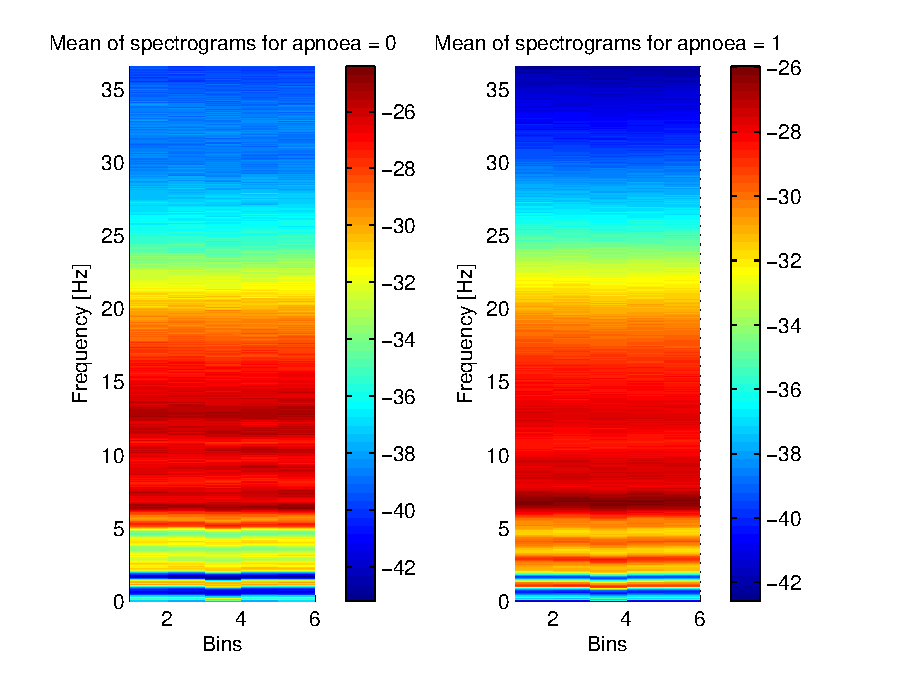
\includegraphics{drawings/spectrogramClassesVisualise.eps}
		\caption{Comparison of the spectrograms of the two classes based on their average spectrogram from the first five records.}
		\label{fig:spectrogramClassesVisualise}
	\end{figure} 
\subsection{Support Vector Machines}
	Firstly, we investigate the case when no kernels are used. Then we will investigate the use of two possible kernels -- polynomial (degree 3) and radial basis function. We will train on the first ten records using the \verb!MATLAB!\textsuperscript{\textregistered}'s function \verb!svmtrain!. Then we will test our trained parameters on the next five records, where we record the accuracy as the ratio of the number of correctly classified annotations over the total number of annotations. We will also record the number of Support Vectors (SVs) because they indicate the generalisation performance.

\subsubsection{No kernels}
	The results of this experiment are shown in Figure \ref{fig:svmExperimentNoKernels} and in Table \ref{table:svmResults}. The accuracy is high, however so is the number of SV's. This indicates that the generalisation guarantee is poor.
	\begin{figure}[htb]
		\centering
		\subfloat[record 11]{%
			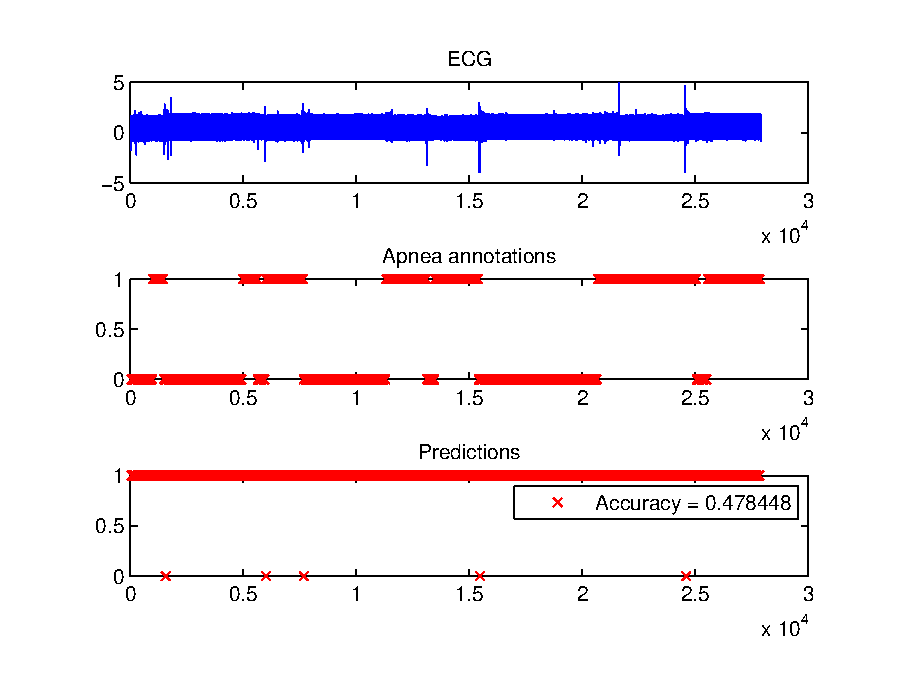
\includegraphics[width=.33\textwidth]{drawings/svm/svmTestNoKernel11}}
		\subfloat[record 12]{%
			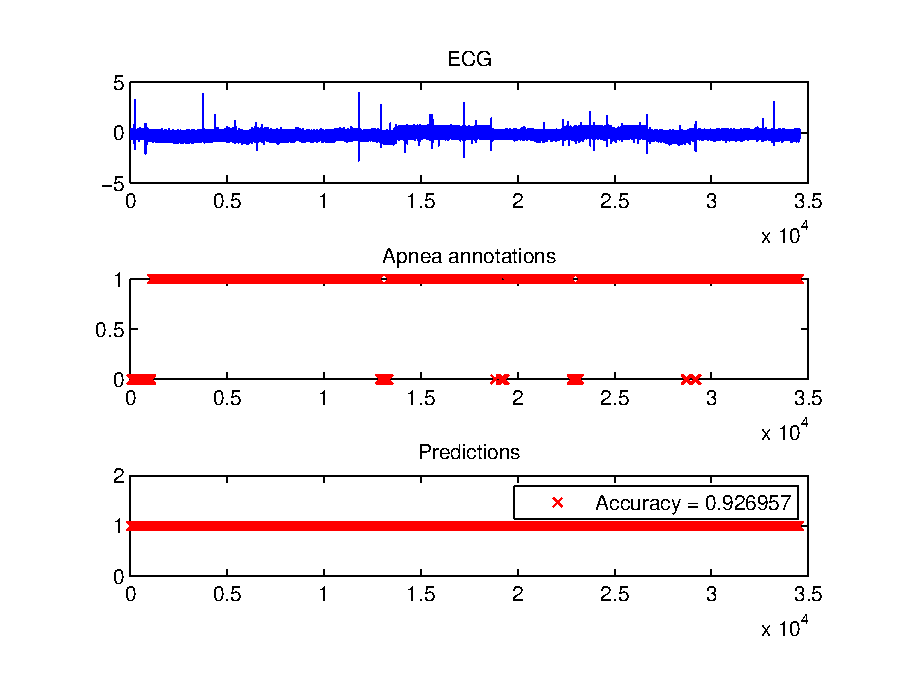
\includegraphics[width=.33\textwidth]{drawings/svm/svmTestNoKernel12}}
		\subfloat[record 13]{%
			\includegraphics[width=.33\textwidth]{drawings/svm/svmTestNoKernel13}} \\
		\subfloat[record 14]{%
			\includegraphics[width=.33\textwidth]{drawings/svm/svmTestNoKernel14}}
		\subfloat[record 15]{%
			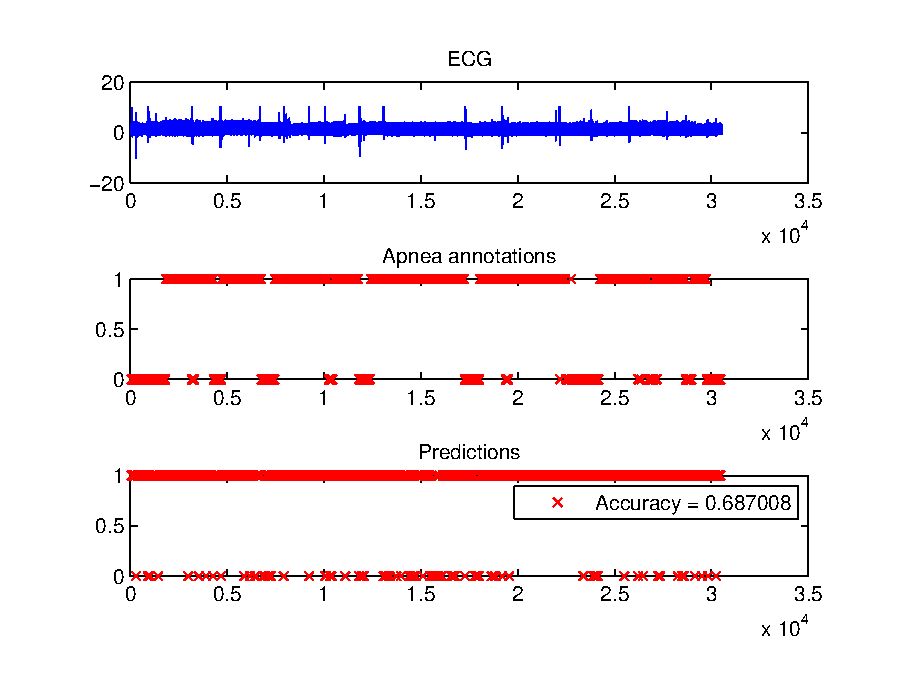
\includegraphics[width=.33\textwidth]{drawings/svm/svmTestNoKernel15}}
		\caption{Performance of no kernels on the test records 11 to 15}
		\label{fig:svmExperimentNoKernels}
	\end{figure}

\subsubsection{Polynomial kernel}
	The results of this experiment are shown in Figure \ref{fig:svmExperimentPoly} and in Table \ref{table:svmResults}. We can see that there is a low number of SVs and high accuracy. This means that the polynomial kernel is likely to perform well on unseen data. If we had more computational resources, we could have used more features (and correspondingly more training data) in order to represent the features better.
	\begin{figure}[!h]
		\centering
		\subfloat[record 11]{%
			\includegraphics[width=.33\textwidth]{drawings/svm/svmTestPoly11}}
		\subfloat[record 12]{%
			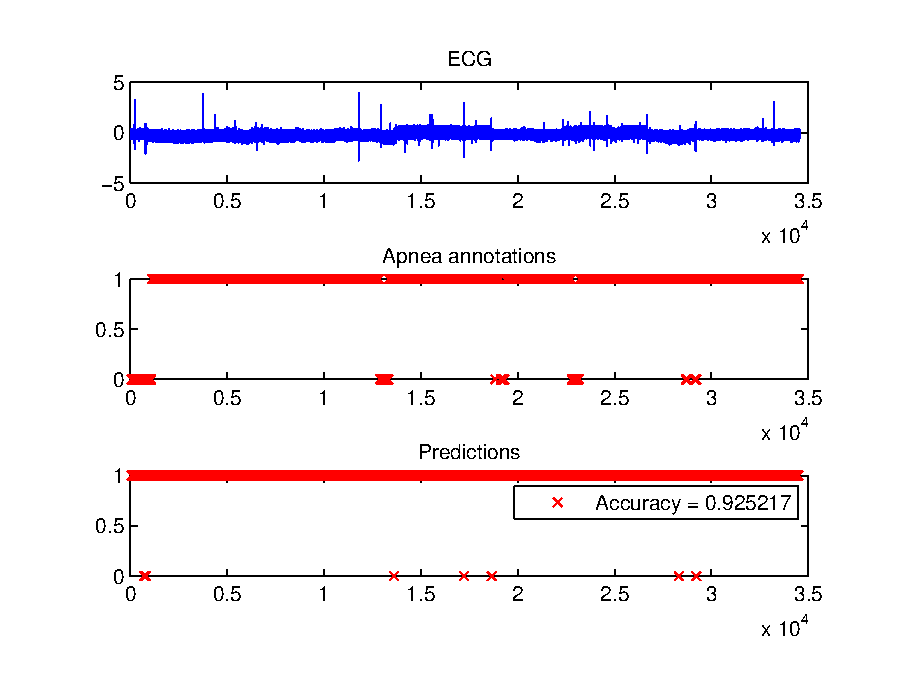
\includegraphics[width=.33\textwidth]{drawings/svm/svmTestPoly12}}
		\subfloat[record 13]{%
			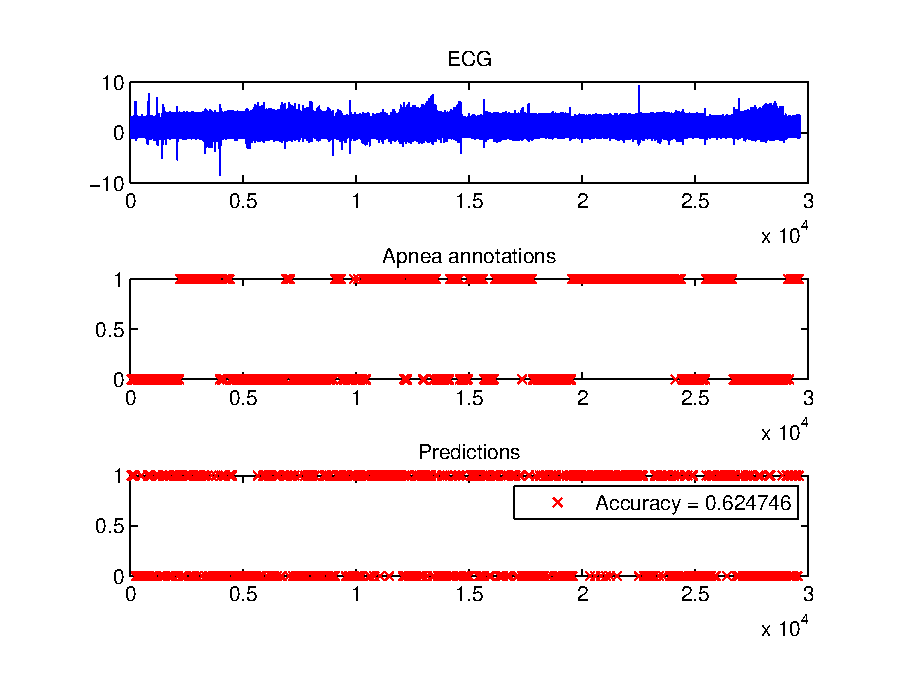
\includegraphics[width=.33\textwidth]{drawings/svm/svmTestPoly13}} \\
		\subfloat[record 14]{%
			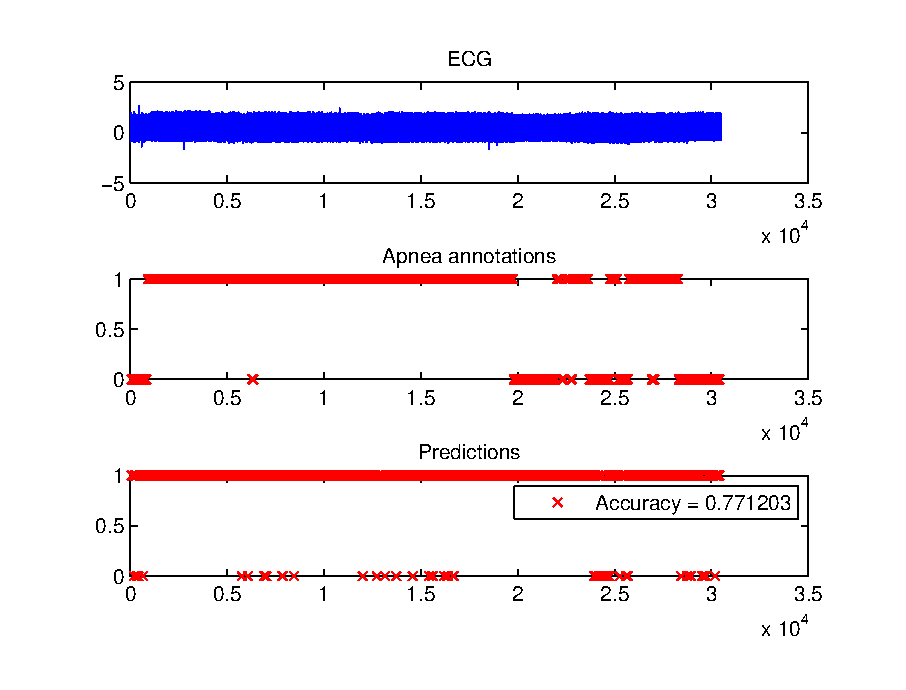
\includegraphics[width=.33\textwidth]{drawings/svm/svmTestPoly14}}
		\subfloat[record 15]{%
			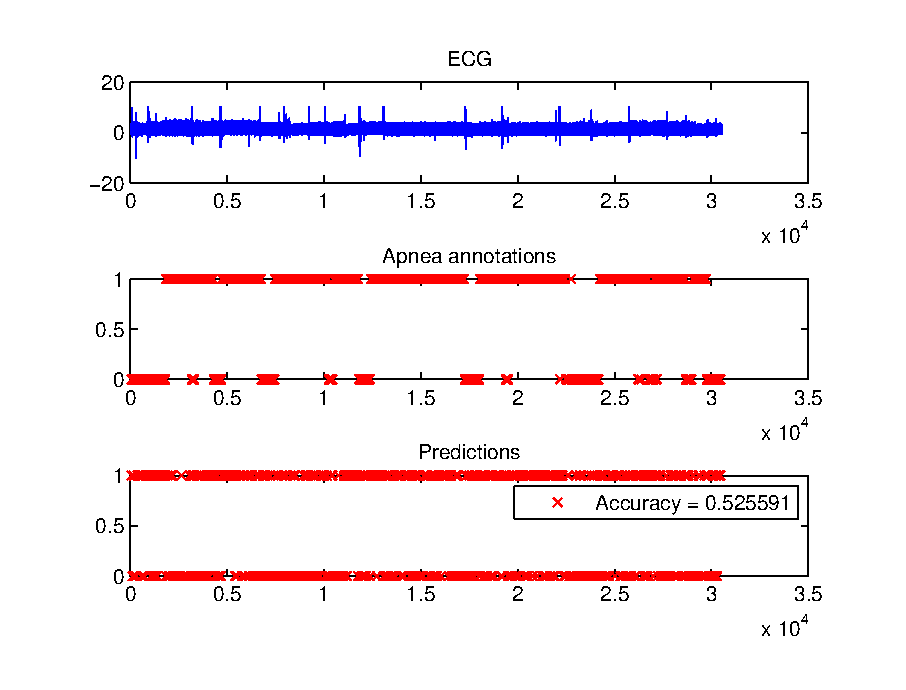
\includegraphics[width=.33\textwidth]{drawings/svm/svmTestPoly15}}
		\caption{Performance of the polynomial kernel on the test records 11 to 15}
		\label{fig:svmExperimentPoly}
	\end{figure}

\subsubsection{Radial basis function kernel}
	The results of this experiment are shown in Figure \ref{fig:svmExperimentRbf} and in Table \ref{table:svmResults}. Similarly to the case of no kernels, the accuracy is high, but so is the number of SV's indicating poor generalisation performance.
	\begin{figure}[!h]
		\centering
		\subfloat[record 11]{%
			\includegraphics[width=.33\textwidth]{drawings/svm/svmTestRbf11}}
		\subfloat[record 12]{%
			\includegraphics[width=.33\textwidth]{drawings/svm/svmTestRbf12}}
		\subfloat[record 13]{%
			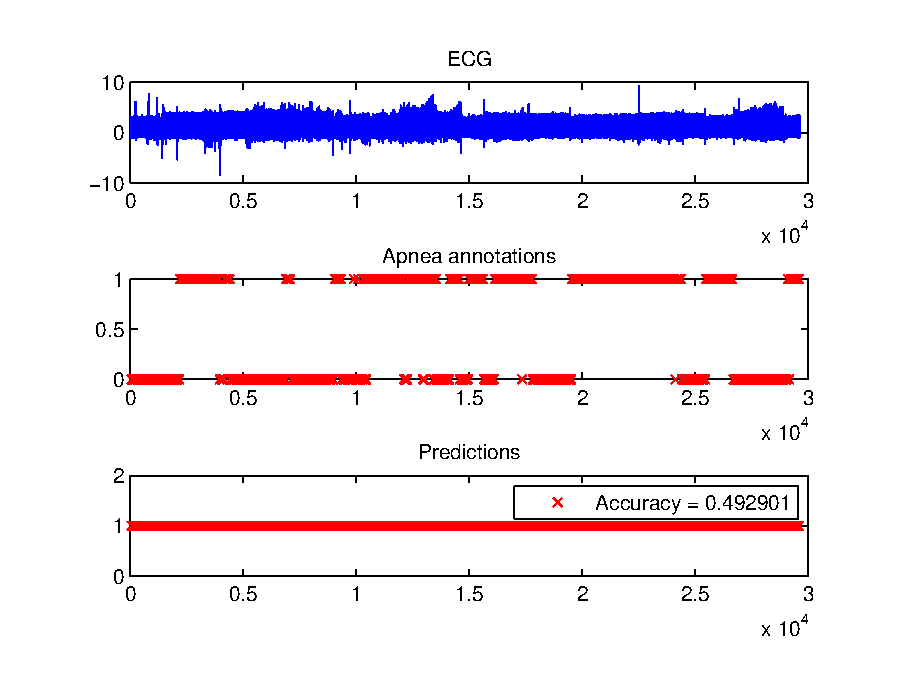
\includegraphics[width=.33\textwidth]{drawings/svm/svmTestRbf13}} \\
		\subfloat[record 14]{%
			\includegraphics[width=.33\textwidth]{drawings/svm/svmTestRbf14}}
		\subfloat[record 15]{%
			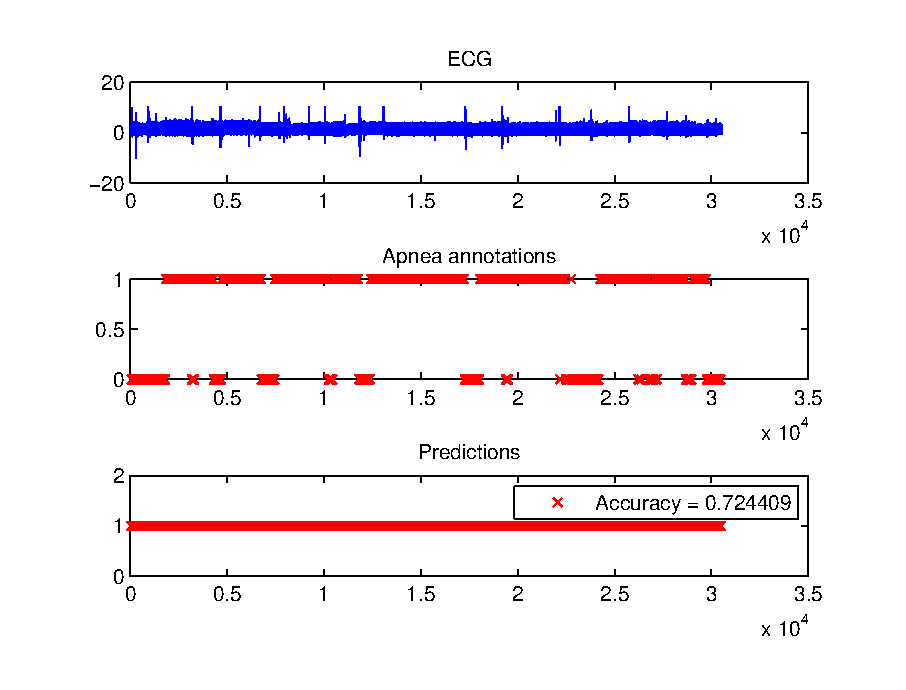
\includegraphics[width=.33\textwidth]{drawings/svm/svmTestRbf15}}
		\caption{Performance of the Radial Basis Function kernel on the test records 11 to 15}
		\label{fig:svmExperimentRbf}
	\end{figure}

\subsubsection{Summary}
	Summary of the performances of the different kernels is shown in Table \ref{table:svmResults}. The polynomial kernel with degree 3 is the most promising in terms of generalisation. All three kernels have similar accuracy. If we had more computational resources, we could have done deeper analysis and tests, e.g. use more principal components to capture as much variance as possible and use more training data (we only used 10 out of 35).
	\begin{table}[h]
		\centering
		\begin{tabular}{@{}lll@{}}
		\toprule
		            & \# SV's (5005 data points) & Average accuracy \\ \midrule
		No kernel   & 3679                       & 0.7116           \\
		Poly kernel & 1879                       & 0.6801           \\
		Rbf kernel  & 4033                       & 0.6814           \\ \bottomrule
		\end{tabular}
		\caption{Summary of performances of different kernels}
		\label{table:svmResults}
	\end{table}
\subsection{Hidden Markov Models (Sachin)}
\label{sec:hmmExperiments-sachin}

Having examined briefly the theory behind Hidden Markov Models, let us now look at how the training was done offline, and analyse some results from subsequent tests. As mentioned earlier, the apnoeatic states are modelled as the hidden states $\{x_t\}_1^T$, and are elements of the binary set $\{0, 1\}$. The observed signal is annotated every K samples (every minute in the case of the PhysioNet data), so we stack all K samples into $\vec y_t \in \mathbb{R}^d$, ($d = K$). Using the packages \verb!pmtk3! and \verb!HMM Toolbox!, the algorithms were implemented in \verb!MATLAB!\textsuperscript{\textregistered}, along with the conditioning of the data using spectrogram and PCA analysis. Again, \verb!MATLAB!\textsuperscript{\textregistered} is used for convenience and the code can be easily converted to \verb!Java! after experimentation and analysis.

The data is read and conditioned as explained in Section \ref{sec:RandCDatainMATLAB}.

We then move on to training and fitting the parameters, using the \verb!pmtk3! and \verb!HMM Toolbox! packages. We then compare the expected hidden states calculated using the \verb!Viterbi Algorithm! with the actual underlying states and determine the accuracy of the HMM model diagnosis.

The parameters are fitted using the \verb!apneaHMMTrain! function shown in Appendix \ref{sec:apneaHMMTrain}, which computes the transitional matrix \verb!A! using

\begin{align}
		A_{ij} & = \frac{\sum_{t = 1}^{T - 1} 1\{x_t = s_i \land x_{t + 1} = s_j\}}{\sum_{t = 1}^{T} 1\{x_t = s_i\}}
\end{align}

and uses Gaussian fitting to calculate the pdfs for the emissions (the \verb!gaussFit! function is used from the \verb!HMM Toolbox! package -- we shall not go into the details on how the function is implemented here). We are left with the outputs \verb!A!, the 2x2 transition matrix, \verb!Mu! and \verb!U!, parameters of the Gaussian pdf fit of the emissions, and \verb!pi!, the initial state distribution.

In order to compare with the test data, we need to read the data specified using \verb!testIndex!, condition it, and use the \verb!Viterbi Algorithm! to calculate the most likely path. This is done in the function \verb!apneaHMMTest!, found in Appendix \ref{sec:apneaHMMTest}. The code for reading and conditioning the data (and plotting the results) has been ommitted as it is similar to that shown before. Once again, functions from `off-the-shelf' packages are used in implementing the \verb!Viterbi Algorithm! and the accuracy of the most likely path is calculated by comparing it to the annotations reflecting the true states. This is done for each test file, and the results are shown below, in Figure \ref{fig:hmmExperiment}. The average accuracy for all 5 test files was found to be 64.1\%.

\begin{figure}[ht]
		\centering
		\subfloat[record 11]{%
			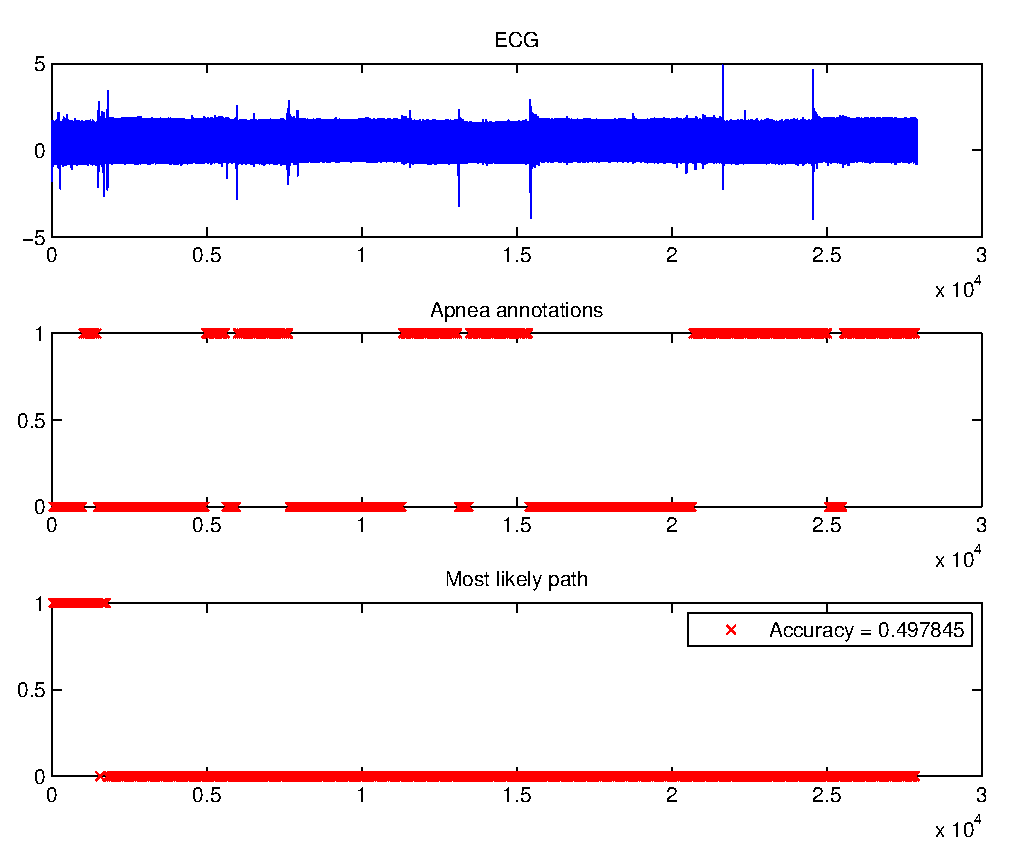
\includegraphics[width=.33\textwidth]{drawings/hmm/hmmTest11}}
		\subfloat[record 12]{%
			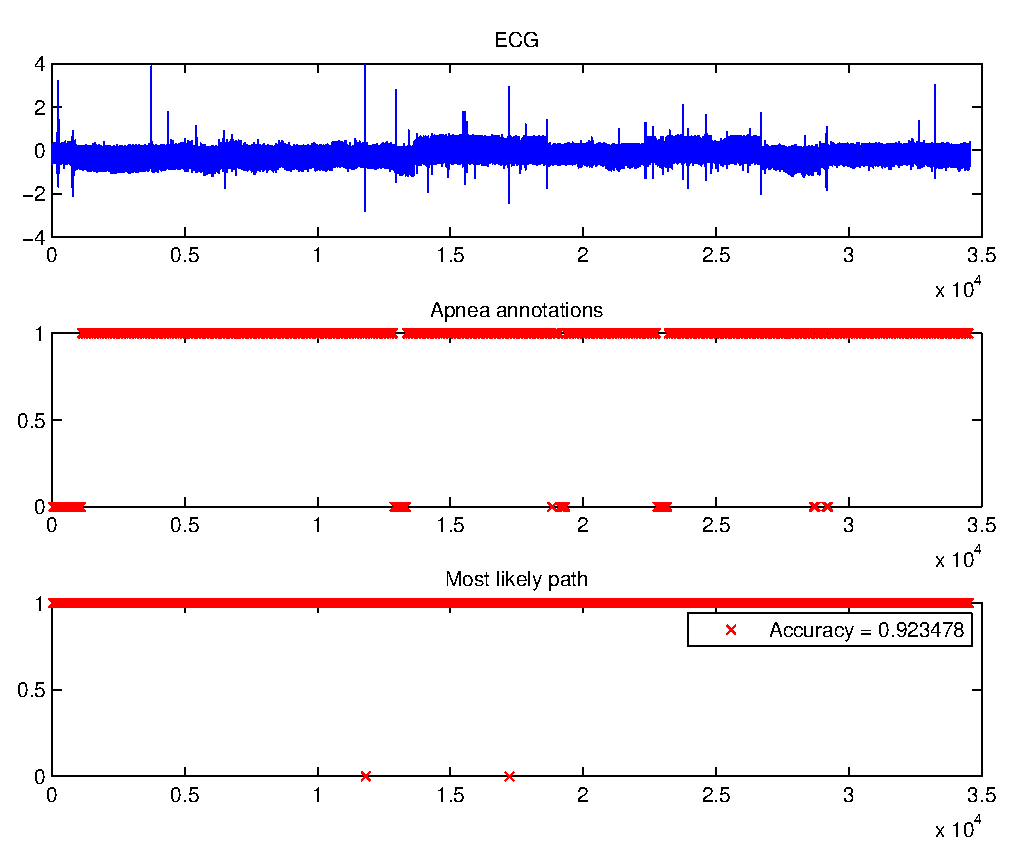
\includegraphics[width=.33\textwidth]{drawings/hmm/hmmTest12}}
		\subfloat[record 13]{%
			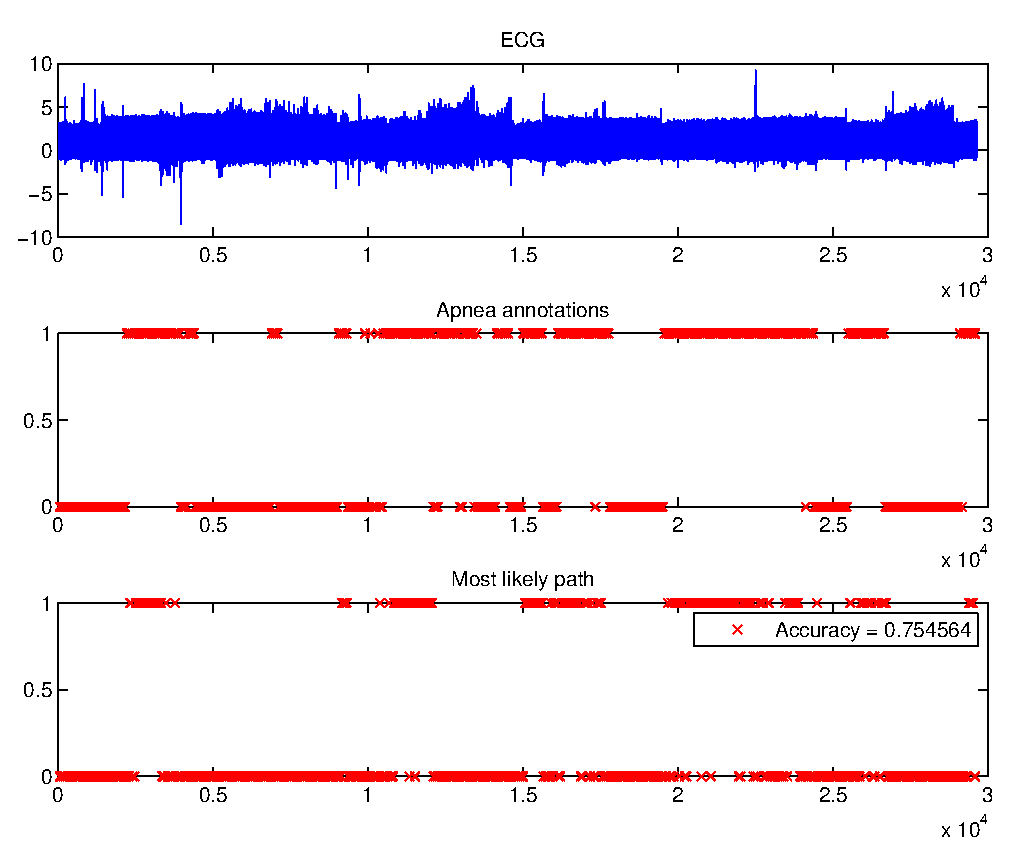
\includegraphics[width=.33\textwidth]{drawings/hmm/hmmTest13}} \\
		\subfloat[record 14]{%
			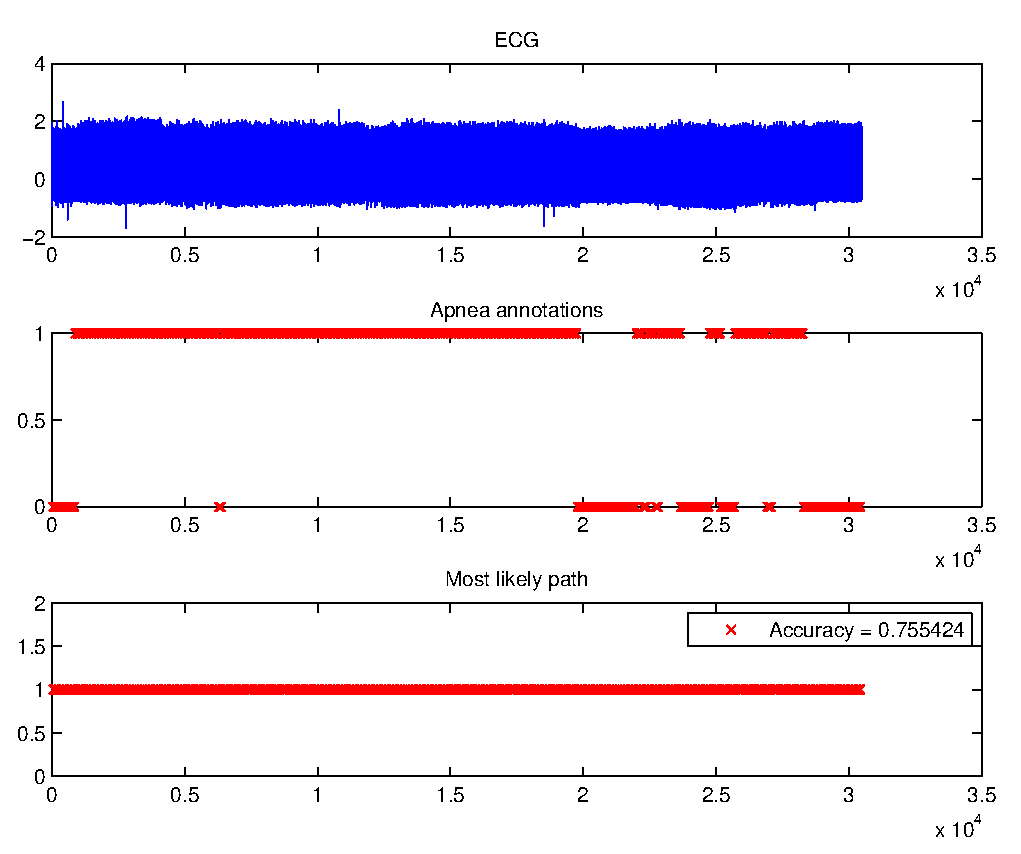
\includegraphics[width=.33\textwidth]{drawings/hmm/hmmTest14}}
		\subfloat[record 15]{%
			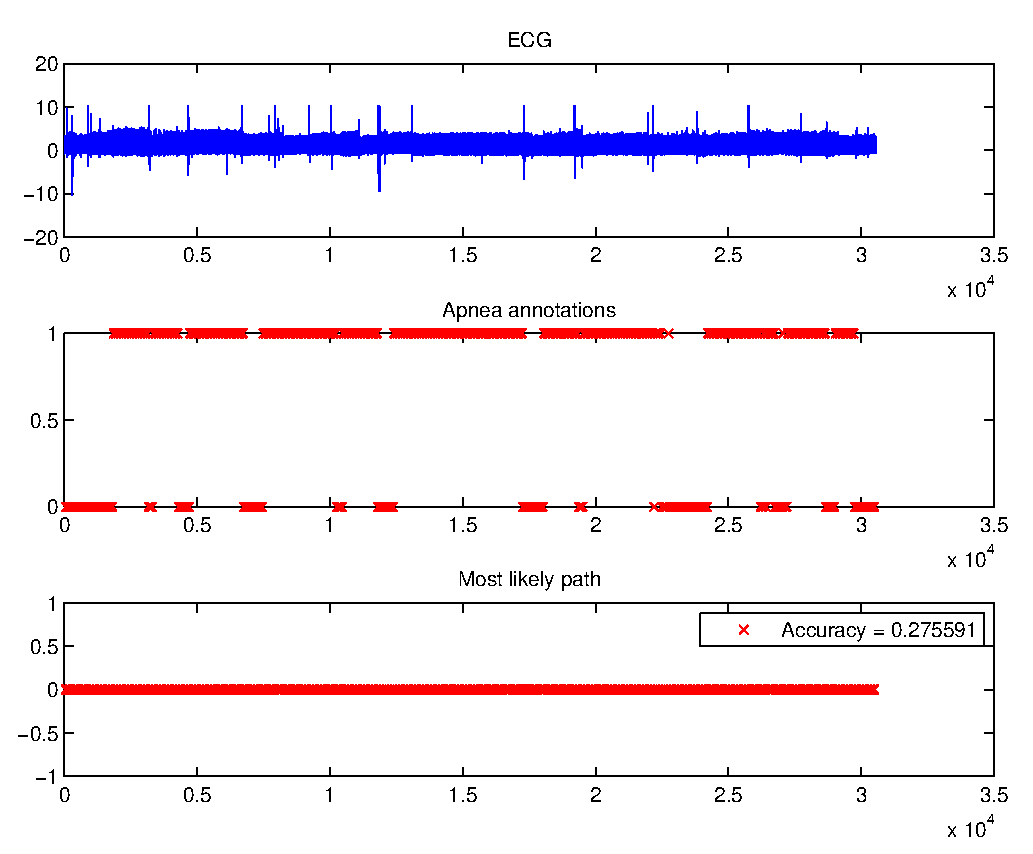
\includegraphics[width=.33\textwidth]{drawings/hmm/hmmTest15}}
		\caption{Performance of HMM model on the test records 11 to 15}
		\label{fig:hmmExperiment}
\end{figure}

\subsection{Summary}

We have seen the implementation of the SVM and HMM models to the PhysioNet data and have calculated the accuracy of both methods in diagnosing apnoea from five records. On the surface, while it may seem that the SVM model provides us with higher accuracy, we feel that the HMM model is more appropriate for use in our app. The accuracy can be improved, firstly, by using more data (we only used 10 of the 35 files for testing) and secondly, by ensuring that the annotations on training and testing data reflect the reality of the patient.

What we have managed to prove here, however, is that diagnosis of OSA using non-invasive techinques is possible if the appropriate machine learning tools are utilised. If more resources were to be invested, an accurate and comprehensive diagnosis can be created in conjunction with the questionnaire.

\newpage
\section{Machine Learning -- Java}
\label{sec:mljava}

\newpage
\section{Designing an Android App}
\label{sec:android-george}
In this section of the report about designing an Android app with the “Android Developer Tools” (ADT) software, there will not be any coding guidance on the basics of Java nor XML. As such, any examples discussed or shown will either have a short explanation or will be simple enough to assume the functionality of the code is evident. The ADT software is used in this project as it facilitates the balance in a simple to use package yet includes more detailed app functionality such as accessing the sound recorder’s buffer. There are many other Android app developing software packages, but none achieve this balance as well. For example the “MIT app inventor” provides basic building blocks for an app but limits the customisation of the code that is an essential element for our audio processing. “appsgeyser.com” is even simpler in providing an app interface for a pre-existing website. However we have decided not to use a web-based approach due to the extra complications from patient security and limitations in excessive data usage in streaming audio to a website.
\subsection{XML and Java sides of ADT}
The “Android Developer Tools” software has a simple architecture for basic apps, which uses XML code to create the user interface of buttons and graphics, and Java code to describe to the phone what each of these items in the XML code does. So for any page of the phone app, there is an XML code called the “layout” with an associated set of Java instructions called a Java “activity”. Whilst it is intuitively easier to consider a visual layout with instructions behind each section, the programming design works much more naturally the other way around, with the Java activity dictating the layout. For this particular app, we need four pages in total. Therefore we need to create a total of four Java activities to describe each page, and each one of these will call an XML layout to attach various commands to.
\subsection{XML IDs}
Each interactive item of the XML layout will have a unique ID, and the Java code will directly link an object to this, which can then be used in the functionality instructions. The following code first assigns the XML button ID “btn\_analyse” to a Java button object called 'btnAnalyse', then informs the phone to carry out the task “startAnalyseActivity()” when it detects that the button has been pressed.
\begin{lstlisting}
btnAnalyse = (Button) findViewById(R.id.btn_analyse);
btnAnalyse.setOnClickListener(new View.OnClickListener() {
public void onClick(View v) {
startAnalyseActivity();
          }
    });
\end{lstlisting}
Our application uses a minimalistic interface and as such there are few XML IDs to work with. Regardless, a convention was established such that each object is labeled by it’s type followed by an underscore, then it’s unique name (for example btn\_analyse as above).
\subsection{Methods}
The task “startAnalyseActivity()” used in the example above is known as a “method” in Java code and is a set of code instructions grouped together under a single name. Not only does this make the code clearer to understand, it also allows repeated sections of code to be called much more simply: just contain all the repeated parts under one method and call that method each time. For these reasons, code for each part of the application functionality is contained in separate methods.
\subsection{Java and android libraries}
The app writer is not expected to write machine level code for the smart phone and is provided with a large array of building blocks for both Java and Android based coding which are contained in “libraries” which must be imported at the start of each activity. For example, the “Android.media.AudioRecord” library is needed to use the phone’s built in microphone, and it provides simple inbuilt methods such as “startRecording()” and “stop()”. Further details of this particularly important library will be discussed later.
\subsection{Structure of an Activity}
Each activity can be divided down into several key blocks that can be explained in the chronological order in which they are seen in the code:
\begin{enumerate}
\item Importing the necessary libraries of methods
\item Declaring the whole activity to create it
\item Declaring any variables and objects that the activity uses
\item Creating the onCreate() task upon which the activity starts running, and in which the core instructions and external methods are called
\item Defining any extra methods used, with their code detailed inside
\end{enumerate}
\subsection{XML writing}
Again, it is not within the scope of this report to comprehensively explain how to code XML, but the code here is very clear to comprehend upon reading each line of code. The “Android Developer Tools” software allows the user to directly edit the XML code, and to also view and edit the layout from a graphical “preview” layout. Note that editing either one of these will update the other in real time. Each object is defined in a block enclosed by < and /> and must contain it’s own ID definition as a minimum. The app’s theme will dictate a large set of default values for any object parameter, so only the physical size and details unique to each object need to be added. This might include unique text for a button or a variation in font for some text – all of which are edited under very clear labels such as “android:fontFamily=…”.
\subsection{XML layouts}
The overall page layout has two main formats: linear layout and relative layout. Relative layout requires each object’s relative position to be labelled in reference to at least one other object with a fixed location and allows objects to be placed alongside each other as well as above and below (effectively two dimensions of freedom). Linear layout is simpler and more constrained in that the objects will be placed in the order they appear in the XML code in one dimension. For this application, linear layout is suitable. Other useful tools here include “<ScrollView/>” which allows all objects within it to be viewed as a scrollable page. This was used on the questionnaire to prevent the questions becoming too small to be readable. It can also be used internally to scroll a subset of objects rather than the whole page.
\subsection{Further XML details}
When defining an object’s size, it’s useful to use adaptable sizes to ensure good results on all devices and screen sizes (as opposed to a set height of 10px for example, which could look small on a tablet but large on a small phone). The two options here are FILL\_PARENT, which makes the object as wide as the object it’s contained in, and WRAP\_CONTENT, which makes the object as wide as necessary to contain all of its components. Using the example of a button width inside an empty android page, FILL\_PARENT would make the button as wide as the screen, and WRAP\_CONTENT would make the button wide enough to include all the button text.
\subsection{Handling Strings}
When creating buttons and other features with text on, the text should be stored in the separate file in “res/values/strings.xml” instead of ‘hardcoding’ it directly into the XML code. Whilst it is less of an issue on a small-scale project such as this, it can become increasingly difficult to find where to change particular items of text in larger projects. Instead we label each part of text from the strings file and reference this ID where it is needed in the code. Then we can quickly find where to change any text in future, or perhaps reuse the same text in multiple buttons or other applications.
\subsection{Java Techniques}
Sharing data between activities can be achieved with a basic technique called “SharedPreferences” which stores any required variable locally in the app. As with many techniques, it requires importing its own class from the android library, and vitally requires the command “editor.commit()” to save the changes before finishing. It is utilised in this application to store the received information from the questionnaire. By restoring the previous stored settings upon the app initialisation, the questionnaire results are then stored on a more permanent basis (I.E when the application has been closed and reopened).
\\ Changing from one activity to another is done using a class called “Intent” which is effectively setting up a requirement for something to happen. In this case the intent will provide the details of the activity to be launched. A button press might then call “startActivity(intent)” which will launch whatever the original intent requested. In this way it can be used as an independent launching mechanism as it is not aware of the details of the intent nor is the intent solely aimed at one target. For example, multiple buttons can launch one action, all acting as effective triggers. In this application, intents are primarily used to launch new activities.
\\ When starting multiple activities, care needs to be taken as to how and when previous activities are closed. Whist it might seem to make sense to have the home page close upon opening a new window, this posed a subtle bug in practice. The pressing of two activity-launching buttons simultaneously causes both of them to open and this is not a significant issue. However, pressing the back button in this format requires launching the “home page” again. Therefore upon exiting one page, a residual page is left open behind the current home page, and upon a few repetitions of this, the app will quickly be running several pages simultaneously. Without exploring in too much depth how to make each activity-launching button press a unique event (such as a mutex-like control), the simplest solution in this case was to allow up to three of the new activity pages to open simultaneously and leave the “home page” unclosed. This limits the total possible number of pages open to four. This is a very unlikely event, and is easily remedied by pressing the back button.
\\ “RadioGroup” buttons are used in the questionnaire section of the app. These provide the advantages of never leaving a blank answer and being instantly comprehendible to any user. Similarly to the buttons, each one has a unique ID to be linked with the Java activity, but they also have unique IDs for each possible selection. The selected answers can then be acted upon by ‘if’ statements using:
\begin{lstlisting}
if (radioOne.getCheckedRadioButtonId() == R.id.radioY1)
  { /* Do action */ } 
\end{lstlisting}
\subsection{Initialising AudioRecord}
It is worth looking in further detail at the AudioRecord android class that we use for the audio input. The initialisation of “new AudioRecord()” uses five parameters, which are explained below:
\begin{itemize}
\item “audioSource” should be set to “1” to default to the inbuilt microphone
\item “sampleRateInHz” should be set to “44100” to guarantee functionality on all devices, however a much lower sample rate would be preferable for the basic application here, and a solution to this is described below.
\item “channelConfig” should be set to “16” for recording sound in MONO rather than STEREO. 
\item “audioFormat” should be set to “2“ for PCM 16bit or “3” for PCM 8bit. This application uses 16bit to ensure functionality on the greatest number of devices possible.
\item “bufferSizeInBytes” is set using an inbuilt method called “getMinBufferSize()”. The inputs to this are the same as parameters 2, 3 and 4 in the AudioRecord initialisation.
\end{itemize}
So the initialisation for the application should look as follows:
\begin{lstlisting}
new AudioRecord(1,44100,16,2,getMinBufferSize(44100,16,2));
\end{lstlisting}
In practice, each input is assigned to a variable that is defined at the top of the code for easy modification and better clarity in the code.
\\ For recording snoring frequencies, a sample rate of as low as 4000Hz would be adequate. The following code solves the earlier discussed issue of minimising the sampling rate. The “getMinBufferSize() is tested on each value added in the for() loop, but as soon as the function returns a positive (hence a valid) bufferSize, the method returns this lowest valid sample rate and “breaks” to finish the method.
\begin{lstlisting}
public int getValidSampleRates() {
  int samplerate = 0;
for (int rate : new int[] {8000, 11025, 16000, 22050, 44100}) {
  int bufferSize = AudioRecord.getMinBufferSize(rate, AudioFormat.CHANNEL_CONFIGURATION_DEFAULT, AudioFormat.ENCODING_PCM_16BIT);
if (bufferSize > 0) {
  samplerate = rate;
  break;}
}
return samplerate };
\end{lstlisting}
\subsection{Progress Wheel}
A progress wheel requires two tasks to be carried out simultaneously – the wheel itself, and the task that has the progress being indicated. This is done with the AsyncTask that allows a background operation to interact with the user interface element: effectively two threads are running and we can allow the UI thread to be updated from the background task. There are four self-explanatory steps in the asynchronous task called onPreExecute, doInBackground, onProgressUpdate and onPostExecute.
\\ To use an example in this app, the “SaveToFileTask” first calls the progress wheel to show on screen with “ProgressDialog.show(…)” in the onPreExecute() step. It then calls the method “audioData.saveData(…)” in the doInBackground() step and finally calls “progressDialog.dismiss()” in onPostExecute() which will clearly indicate that the data has been saved. Note that the onProgressUpdate step is not used, as we do not have a use for updating the UI whilst running the background task. This might, for example, be used to change the text on the progress wheel to indicate when a second task is being carried out had one been present.
\subsection{GraphView}
GraphView is an additional library available for Android and is particularly useful for an audio application that looks at sound intensities. 
\subsection{Other Platforms}
Apple provide their own libraries similar to those in android, that provide quickly usable methods and hardware capability to a developer. The sleep apnea app has suitably simple components that can be recreated on Apple’s iOS like for like if required. This section of the report will quickly overview the techniques to do this, but will also detail other available tools and how they might be used more to create a more effective native app in iOS. This section will not detail any code, purely discussion of the available libraries and tools.
\subsection{Xcode}
Xcode is the free software available in the Apple App Store that contains all the necessary prototyping and developing tools to produce an application on iPhone, iPad and Mac. Code can be written in Objective-C, C and a whole multitude of other languages with interpreters to adapt them. Xcode provides an Integrated Development Environment (IDE), compiler with inbuilt “bug” finding, an iOS simulator to virtually test the app amongst other things. Similarly to the Android Developer Tools, memory analysis, CPU profiling and general performance tracking is all included. This would provide a very suitable basis to build our app from.
\subsection{AVAudioRecord Library}
The most important library to consider here is the inbuilt capabilities of the audio recording. A handful of the more unique and interesting classes will be discussed here:
\begin{itemize}
\item recordAtTime:forDuration: This flexibility in setting the start time to record and the duration of each recording could be applied for a few things. Firstly the start time could be set such to greatly increase the chance of the user being asleep as the recording starts. It could also be used as a basic way to reduce background noise if, perhaps, the user’s sleeping area experienced background noise from parties or traffic until a set time in the evening. Likewise, limiting the duration of the recording could ensure results aren’t skewed from noise of waking up and manually turning the app off. The app could select a key range of hours in the night that maximises the probability of apnea detection and minimises the chance of background noise. Note that this could also be manually implemented in the Android version which is discussed later.
\item averagePowerForChannel This is one of two values provided in the Audio Level Metering section of the library. This could provide a very simple technique to implement a switching state model with perhaps three defined ranges of audio powers. Recording the average power for the channel (in our case there is only one channel in MONO recording) roughly twice per second would provide an array which would accurately reflect the volume of the sleeping user. “Band two” would represent the standard snoring volume observed in almost all sufferers of sleep apnea and would be the expected volume level for the user. “Band one” would be very low audio power indicative that the sleeper’s throat is blocked and an apnea is occurring. “Band three” would represent high audio power, interpreted as the loud snorting very commonly experienced after an apneic episode as the sleeper unblocks their throat. Clearly such a monitoring system would produce very small file sizes, which is a very desirable aim in audio recording based software (in this case, audio isn’t being saved directly to a file, only monitored for power values). This technique doesn’t lend itself well to machine learning techniques due to the lack of precision in the recorded data – features aren’t defined nearly as well as more fully sampled techniques.
\item peakPowerForChannel is the other value provided by the Audio Metering section and whilst not being as directly applicable, could be useful when used in conjunction with averagePowerForChannel. From simple logical reasoning, noise is much harder to detect when the precision of the system is low like the technique suggested above. peakPowerForChannel could therefore be used to calibrate this technique. A short recording of the background noise in controlled quiet conditions could calibrate the allowable background noise for “band one” in the above example, whilst the user recording a faked snort sound could provide a rough expectation for the power to be expected at “band three”. From this, unexpected audio power levels can be rejected or handled differently from the normal operational audio power.
\end{itemize}
\chapter{Conclusion (Sachin)}
\label{ch:conclusion}
 
Obstructive Sleep Apneoa (OSA) is a serious and prevalent condition that affects many middle-aged people, and many of them remain undiagnosed, leading to poor sleep and a reduced quality of life. The current diagnosis solutions offered by the NHS are relatively expensive and inconvenient, and there is a need in the market for a way to check for OSA without having to spend a lot of time, money or effort. The easiest way to provide for this need would be through a smartphone application that would utilise machine learning to diagnose OSA from the user's audio sleep data.

After proving that there is a need and potential market for a mobile app that is able to provide a preliminary diagnosis of OSA, we moved on to first develop a method of diagnosis without using machine learning, to use as a backup and to familiarise ourselves with sleep data. We created a simple method of diagnosis in \verb!MATLAB!\textsuperscript{\textregistered} using power thresholds and variance analysis. This method was able to provide us with an output of 1s or 0s, highlighting different time periods when the user experiences apneoa. We then tested the simple method on a 7 minute audio file obtained from the internet, of a real OSA patient.

We then moved on to research several machine learning techniques that could be used in our app, and identified Support Vector Machines (SVM) and Hidden Markov Models (HMM) as being suitable in our case. We built the models in \verb!MATLAB!\textsuperscript{\textregistered} and ran tests using data obtained from PhysioNet to test the accuracy of both models. We presented the results and argued in Section \ref{sec:mlExperimentsSummary} that the HMM model would be better suited for the purpose of diagnosing OSA from temporal data. 
More importantly, what we were able to show was that if the appropriate model is used, OSA can be accurately diagnosed using only a mobile application on a smartphone and there is the potential to develop and launch it as a complementary service to the current NHS diagnosis and treatment service for OSA. This would save even more time and resources for doctors as the NHS approved questionnaires can be easily performed through the app even before meeting the GP.

In order to improve the accuracy of the diagnosis further, we need to improve both the quality and quantity of testing and training data. Firstly, using audio data (instead of the ECG data that we used in our initial experiments) would provide better applicability to the smartphone. Secondly, improving the quality, in terms of better annotations and multiple annotations by healthcare professionals to ensure accuracy of labelling would improve the accuracy of the model. Thirdly, simply providing more data for the model to estimate the parameters more accurately would, over time, make the app much better than it already is at identifying OSA in users. Lastly, the models we have developed can always be improved upon as well, as shown in Section \ref{sec:mlExperimentsSummary}.

We conclude with the assertion that the implementation and use of the mobile app we have developed would benefit the general public greatly, and also provide many benefits for healthcare professionals as well. We hope that further work will be done in this area to improve and refine the process, such that we finally find an app in the open market.

\appendix
\chapter{Code for the simple model}
\label{ch:simpleCode}

\section{Main script -- simple.m}
\label{sec:simple}
\begin{lstlisting}
% Reading data
clear all;
close all;
FILENAME = 'signal.wav';
[YRaw,f] = audioread(FILENAME) ;
TMAX = length(YRaw) / f;

% Sampling data because we don't need very high resolution
scale = 20;
for i = 1:(length(YRaw) / scale)
    Y(i) = 0.5 * (YRaw(i * scale, 1) + YRaw(i * scale, 2));
end

% Plots sampled data
figure;
plot(Y);
title('Sleep signal');

% Calculates and plots frequency
N = length(Y);
Yf = fft(Y,N);
freq = ((0:1/N:1-1/N)*f).'; % Frequency vector;

% Plot spectrum.
plot(freq,abs(Yf)) 
title('Amplitude Spectrum of y(t)')
xlabel('Frequency (Hz)')
ylabel('|Y(f)|')

% Calculates and plots the power
power = Y.^2;

% Apnea detection
sensitivityMean = 0.01;
interval = 3;
sensitivityVar = 5e-2;
windowSize = 20;
apnea = detectApnea(power, TMAX, sensitivityMean, interval);
apneaVar = detectApneaVar(power , TMAX , sensitivityVar , windowSize);
\end{lstlisting}

\section{Detecting apnoea -- detectApnea.m}
\label{sec:detectApnea}
\begin{lstlisting}
function apnea = detectApnea(Y, TMAX, sensitivityMean, interval)
    n = length(Y); % No. of samples
    sampleInterval = round(n / TMAX * interval); % Minimum no. of consecutive samples that should be below threshold for apnea
    apnea = zeros(1, n); % Generate a vector that will contain either zeros or ones to show where apnea is
    
    threshold = mean(Y) / sensitivityMean;
    
    nBelowThreshold = 0; % Number of sample points below the threshold in a row.
	for i = 1:n
        if Y(i) <= threshold
            nBelowThreshold = nBelowThreshold + 1; % Increase # of sample points below the threshold in a row
        else % We see a point that is above threshold.
            if nBelowThreshold >= sampleInterval % Condition for which we classify apnea.
                for j = max((i - nBelowThreshold), 1):(i - 1) % Loop through the last 'nBelowThreshold' points. Making sure (i - nBelowThreshold) doesn't go below 1 (otherwise error).
                    apnea(j) = 1;
                end
            else
                for j = max((i - nBelowThreshold), 1):(i - 1)
                    apnea(j) = 0;
                end
            end
            nBelowThreshold = 0;
        end
    end
end
\end{lstlisting}

\section{Detecting apnoea using the `variance' method -- detectApneaVar.m}
\label{sec:detectApneaVar}
\begin{lstlisting}
function apnea = detectApneaVar (Y , TMAX , sensitivityVar , windowSize)
n = length (Y);
apnea = zeros (1 , n);

% Calculate variance of whole signal (as a yardstick)
variance = var(Y) ;
maxVariance = variance / sensitivityVar;

% Calculate the variance through a moving window
twindow = [1:windowSize ; Y( 1:windowSize )]; % This vector contains the locations of the moving window

for i = 1:(n - windowSize)
    sigma2 = var( twindow(2, :) );
    
    if sigma2 > maxVariance 
        apnea(1 , twindow(1,:) ) = 1;
    end
    
    twindow(1,:) = twindow(1,:) + 1; % Update the window for the next round of variance calculations
    twindow(2,:) = Y ( twindow(1,:) );
end
\end{lstlisting}
\chapter{Code for reading data -- readData.m}
\label{ch:readData}
\begin{lstlisting}
function [O, q, time, signal, annTime] = readData(fileIndex, keepSignal)
% Reads data from indices specified in the vector fileIndex and returns
%   O = observations, merged together [TxD]
%   q = latent states, 1-0 for apnea-nonapnea [Tx1]
% Inputs
%   fileIndex = vector of file indices to read
%   keepSignal = keep signal and time for plotting purposes (set to 1 or 0)
    
    disp('Reading and conditioning data...');
    filenames = getFilenames();
    
    lastTime = 0;
    annTimeLast = 0;
    time = []; % time
    signal = []; % signal
    annTime = []; % timestamps of annotations
    q = []; % latent states
    O = []; % observations
    for i = fileIndex
        filename = cell2mat(filenames(i));
        disp(sprintf('\tProcessing file %d: %s...', i, filename));
        
        [timeTemp, signalTemp, freq] = rdsamp(filename); % reads the signal
        [annTimeTemp, type] = rdann(filename,'apn'); % reads annotations
        type = (type == 'A');

        %% Conditioning data
        annTimeTemp = [1; annTimeTemp];
        q = [q; type]; % latent states
        for i = 1:length(type)
            O = [O; signalTemp((annTimeTemp(i) + 1):annTimeTemp(i + 1))'];
        end
        
        if keepSignal
            nObs = annTimeTemp(end);
            time = [time; timeTemp(1:nObs) + lastTime + 0.01];
            annTime = [annTime; annTimeTemp(2:end) + annTimeLast];
            signal = [signal; signalTemp(1:nObs)];
            lastTime = time(end);
            annTimeLast = annTime(end);
        end
    end
    if ~keepSignal
        signal = [];
        time = [];
    end
end
\end{lstlisting}
\chapter{Code for data conditioning}
\section{Transforming to spectrogram space -- transformSpectrogram.m}
\label{sec:transformSpectrogram}
\begin{lstlisting}
function [OTransformed, qTransformed] = transformSpectrogram(O, q)
% O = matrix of T D-dimensional observations [TxD]
% q = vector of T hidden states [Tx1]
% OTransformed = spectrograms after transformation and cut-off [T'xD']
% qTransformed = hidden states after cut-off [T'x1]

    [T, D] = size(O);

    freq = 100;
    nBinsPerAnn = 6; % number of bins per annotation
    window = D / 2; % length of window
    nOverlap = window - D / nBinsPerAnn;
    OBig = reshape(O', 1, T * D);
    [Ss, Fs, Ts, Ps] = spectrogram(OBig, window, nOverlap, [], freq); % time on x axis, freq on y axis
    
    timeCutOff = (T - 1) * nBinsPerAnn;
    freqCutOff = 1500;
    Ps = Ps(1:freqCutOff, 1:timeCutOff);

    OTransformed = reshape(Ps, nBinsPerAnn * size(Ps, 1), T - 1)';
    qTransformed = q(1:(T - 1));
end
\end{lstlisting}

\section{Calculating PCA parameters -- pcaCalc.m}
\label{sec:pcaCalc}
\begin{lstlisting}
function [PCoef, PVec, xMean, xVar] = pcaCalc(x, k)
% Calculates the PCA parameters to reduce D-dimensional vectors stored in x
% [NxD] to K-dimensional vectors stored in y [NxK]
%   PCoef = vector of eigenvalues (variances)
%   PVec = k principal bases stored in k columns [DxK]
%   xMean = mean of data x (for future normalisation purposes)
%   xVar = var of data x (for future normalisation purposes)
    
    % Normalise
    xMean = mean(x);
    xVar = var(x, 1);
    x = bsxfun(@minus, x, xMean);
    x = bsxfun(@rdivide, x, sqrt(xVar));
    
    % PCA
    [PCoef, PVec] = pca(x); % DxD, with i-th column being the i-th principal component (from PMTK3 package)
    PVec = PVec(:, 1:k); % consider only the first k components
end
\end{lstlisting}

\section{Reducing dimensions using PCA -- pcaTransform.m}
\label{sec:pcaTransform}
\begin{lstlisting}
function y = pcaTransform(x, PVec, xMean, xVar)
% Reduces dimensions of D-dimensional vectors in x [NxD] to K-dimensional
% vectors stored in y [NxK] using PCA parameters

    % Normalise
    x = bsxfun(@minus, x, xMean);
    x = bsxfun(@rdivide, x, sqrt(xVar));
    
    % PCA
    y = x * PVec;
end
\end{lstlisting}
\chapter{Code for Support Vector Machines (Tuan Anh)}
\label{ch:SVMCode}

\section{Main script -- apneaSVM.m}
\label{sec:apneaSVM}
\begin{lstlisting}
trainIndex = 1:10;
testIndex = 11:15;

%% Reading and conditioning data
[X, Y, time, signal, annTime] = readData(trainIndex, 1); % X = input, Y = output

%% Transform spectrogram
[XTransformed, YTransformed] = transformSpectrogram(X, Y);

%% PCA
disp('PCA...');
k = 100; % take k principal components only
[PCoef, PVec, XMean, XVar] = pcaCalc(XTransformed, k);
XPca = pcaTransform(XTransformed, PVec, XMean, XVar);

%% SVM
options = optimset('MaxIter', 1e6);
SVMStructPoly = svmtrain(XPca, YTransformed, 'kernel_function', 'polynomial', 'polyorder', 3, 'options', options); % poly kernel
% SVMStructRbf = svmtrain(XPca, YTransformed, 'kernel_function', 'rbf', 'options', options); % rbf kernel
% SVMStruct = svmtrain(XPca, YTransformed, 'options', options); % no kernel

%% Comparing with test data
apneaSVMTest(SVMStructPoly, PVec, XMean, XVar, testIndex);
\end{lstlisting}

\section{Test script -- apneaSVMTest.m}
\label{sec:apneaSVMTest}
\begin{lstlisting}
function apneaSVMTest(SVMStruct, PVec, XMean, XVar, testIndex)
    disp('Comparing with test data...');
    accuracySum = 0;
    for i = testIndex
        %% Read data
        [XTest, YTest, timeTest, signalTest, annTimeTest] = readData(i, 1);
        
        %% Transform spectrogram
        [XTest, YTest] = transformSpectrogram(XTest, YTest);
        
        %% PCA
        XTest = pcaTransform(XTest, PVec, XMean, XVar);

        %% SVM Classify
        YPredict = svmclassify(SVMStruct, XTest);
        
        accuracy = sum(YPredict == YTest) / length(YTest)
        accuracySum = accuracySum + accuracy;
        
        %% Plotting data
        ...
    end
    avgAccuracy = accuracySum / length(testIndex)
end
\end{lstlisting}
\chapter{Code for Hidden Markov Models (Sachin)}
\label{ch:HMMCode}

\section{Main script -- apneaHMM.m}
\label{sec:apneaHMM}
\begin{lstlisting}
trainIndex = 1:10;
testIndex = 11:15;

%% Reading and conditioning data
[Y, X] = readData(trainIndex, 0); % Y = observations, X = latent states.
N = 2; % number of states: apnea-noapnea
S = [0; 1]; % set of possible states

%% Transform spectrogram
[YTransformed, XTransformed] = transformSpectrogram(Y, X);

%% PCA
disp('PCA...');
k = 100; % take k principal components only
[PCoef, PVec, YMean, YVar] = pcaCalc(YTransformed, k);
figure;
plot(cumsum(PCoef)/sum(PCoef));
YPca = pcaTransform(YTransformed, PVec, YMean, YVar);

%% Fitting parameters
[A, Mu, U, pi] = apneaHMMTrain(XTransformed, YPca, N, S);

%% Comparing with test data
apneaHMMTest(A, Mu, U, pi, PVec, YMean, YVar, N, testIndex);
\end{lstlisting}

\section{Training script -- apneaHMMTrain.m}
\label{sec:apneaHMMTrain}
\begin{lstlisting}
function [A, Mu, U, pi] = apneaHMMTrain(q, O, N, S)
    [T, D] = size(O); % dimension of observations & number observations

    % Transitional matrix A
    disp('Fitting transitions...');
    A = zeros(N);
    for i = 1:N
        for j = 1:N
            transitionsFromSiToSj = 0;
            transitionsFromSi = 0;
            for t = 1:(T - 1)
                transitionsFromSiToSj = transitionsFromSiToSj + (q(t) == S(i) && q(t + 1) == S(j));
                transitionsFromSi = transitionsFromSi + (q(t) == S(i));
            end
            A(i, j) = transitionsFromSiToSj / transitionsFromSi;
        end
    end

    % Estimate Gaussian parameters
    disp('Fitting emissions...');
    Mu = zeros(D, N); % means
    U = zeros(D, D, N); % covariances
    for j = 1:N
        x = O(q == S(j), :);
        model = gaussFit(x); % from PMTK3 package
        Mu(:, j) = model.mu;
        U(:, :, j) = model.Sigma;
    end

    % Estimate HMM parameters
    pi = [0.5; 0.5];
end
\end{lstlisting}

\section{Test script -- apneaHMMTest.m}
\label{sec:apneaHMMTest}
\begin{lstlisting}
function apneaHMMTest(A, Mu, U, pi, PVec, YMean, YVar, N, testIndex)
    disp('Comparing with test data...');
    accuracySum = 0;
    for i = testIndex
        %% Read data
        [YTest, XTest, timeTest, signalTest, annTimeTest] = readData(i, 1);
        
        %% Transform spectrogram
        [YTest, XTest] = transformSpectrogram(YTest, XTest);
        
        %% PCA
        YTest = pcaTransform(YTest, PVec, YMean, YVar);

        %% Most likely path (Viterbi)
        disp(sprintf('\tCalculating the most likely path...'));
        B = [];
        for j = 1:N
            B(j, :) = gaussian_prob(YTest', Mu(:, j), U(:, :, j)); % from HMM Toolbox
        end
        path = viterbi_path(pi, A, B) - 1; % from PMTK3 package
        
        accuracy = sum(path == XTest') / length(XTest)
        accuracySum = accuracySum + accuracy;
        %% Plotting data ...
    end
    avgAccuracy = accuracySum / length(testIndex)
end
\end{lstlisting}
% \chapter{Division of labour}
\label{ch:divisionOfLabour}
The work has been split in the following way.

\begin{itemize}
	\item George Cochrane has written \fullref{ch:app}, and \fullref{sec:android-george}.
	\item Tuan Anh Le has written \fullref{sec:mltheory-ta}, \fullref{sec:conditioningExperiments-ta}, \fullref{sec:dataVisualisation-ta}, \fullref{sec:svmExperiments-ta}, \fullref{sec:mljava}, \fullref{ch:dataConditioningCode} and \fullref{ch:SVMCode}.
	\item Sophie Louth has written \fullref{ch:medicalInfo}, \fullref{sec:medicalneed-sophie}, \fullref{sec:diagnosticMethods-sophie}, \fullref{sec:signsAndSymptoms-sophie}, \fullref{sec:questionnaire-sophie}, and \fullref{sec:audio-sophie}
	\item Sachin Mylavarapu has written \fullref{sec:economics-sachin}, \fullref{sec:simple-sachin}, \fullref{sec:hmmExperiments-sachin}, \fullref{sec:mlExperimentsSummary}, \fullref{ch:simpleCode}, \fullref{ch:readingDataCode}, and \fullref{ch:HMMCode}.
\end{itemize}

\bibliographystyle{plain}
\bibliography{bibliography/tuananh,bibliography/sachin,bibliography/george,bibliography/sophie}
\end{document}